% concatenated from spd-opinf.tex, packages.tex, commands.tex, burgers.tex, nonlinear-cdr.tex, nonlinear-heat.tex, air-flame.tex, torsion.tex
%\documentclass{article}
\documentclass[3p,computermodern,11pt]{elsarticle}
\usepackage{fullpage}
%\usepackage{algorithm,algorithmic}
%\usepackage[ruled]{algorithm2e}
\usepackage{booktabs} % For better table formatting
\usepackage{algorithm}
\usepackage{algorithmic}
%\usepackage{cite}
\usepackage[utf8]{inputenc}
\usepackage[english]{babel}
\usepackage{amsmath,amsfonts,amssymb,amsthm}
\usepackage{ulem}
\newtheorem{theorem}{Theorem}[section]
\newtheorem{lemma}{Lemma}[section]
\newtheorem{proposition}{Proposition}[section]
\newtheorem{corollary}{Corollary}[theorem]
\newtheorem{remark}{Remark}[section] 
\usepackage{color}
\usepackage{xcolor}
\usepackage{mathtools}
\usepackage[titletoc,title]{appendix}
%======
\usepackage{float}
%\usepackage{wrapfig,blindtext}
\usepackage{graphicx} % to include images
\usepackage{epstopdf} % to convert eps to pdf
\usepackage{caption}[font=small,skip=-2pt]
\usepackage{subcaption}[font=small,skip=-2pt]
\usepackage{pdfpages}
\usepackage{comment}
\usepackage{tabularx}
\usepackage{listings}

\usepackage{hyperref}
\hypersetup{
    colorlinks=true,
    linkcolor=blue,
    filecolor=magenta,      
    urlcolor=cyan,
}
\urlstyle{same}
%\setlength{\belowcaptionskip}{-5pt}
%\usepackage{sfmath} 

\usepackage{tikz}
\usetikzlibrary{positioning, fit, arrows.meta, shapes}
\newcommand{\empt}[2]{$#1^{\langle #2 \rangle}$}
\usetikzlibrary{
  arrows.meta, % for Straight Barb arrow tip
  fit, % to fit the group box around the central neurons
  positioning, % for relative positioning of the neurons
}
\tikzset{
  neuron/.style={ % style for each neuron
    circle,draw,thick, % drawn as a thick circle
    inner sep=0pt, % no built-in padding between the text and the circle shape
    minimum size=3.5em, % make each neuron the same size regardless of the text inside
    node distance=1ex and 2em, % spacing between neurons (y and x)
  },
  group/.style={ % style for the groups of neurons
    rectangle,draw,thick, % drawn as a thick rectangle
    inner sep=0pt, % no padding between the node contents and the rectangle shape
  },
  io/.style={ % style for the inputs/outputs
    neuron, % inherit the neuron style
    fill=gray!15, % add a fill color
  },
  conn/.style={ % style for the connections
    -{Straight Barb[angle=60:2pt 3]}, % simple barbed arrow tip
    thick, % draw in a thick weight to match other drawing elements
  },
}
\numberwithin{equation}{section}

\lstdefinestyle{nnopinf}{
  language=Python,
  basicstyle=\ttfamily\small,
  keywordstyle=\color{blue!60!black},
  commentstyle=\color{green!50!black},
  stringstyle=\color{orange!70!black},
  backgroundcolor=\color{gray!10},
  frame=single,
  rulecolor=\color{gray!60},
  breaklines=true,
  showstringspaces=false
}

\newcommand{\adg}[1]{\textcolor{cyan}{ADG: #1}}

%\newcommand{\forcing}{\mathbf{b}}
\newcommand{\nnopinf}{NN-OpInf}
\newcommand{\one}{\boldsymbol 1}
\newcommand{\HTwo}{\mathrm{H}_2}
\newcommand{\OTwo}{\mathrm{O}_2}
\newcommand{\HTwoO}{\mathrm{H}_2\mathrm{O}}
\newcommand{\code}[1]{{\ttfamily\color{black} #1}}
\newcommand{\forcingScalar}{b}
\newcommand{\reducedOperatorLinear}{\hat{\mathbf{A}}}
\newcommand{\reducedOperatorQuadratic}{\hat{\mathbf{H}}}
\newcommand{\range}[1]{\mathrm{range}\left(#1\right)}

\newcommand{\nBfgsSteps}{n_{\mathrm{lbfgs}}}

\newcommand{\lhs}{\boldsymbol z}
\newcommand{\inputs}{\boldsymbol u}
\newcommand{\reducedLhs}{\dot{\hat{\state}}}
\newcommand{\reducedState}{\hat{\state}}
\newcommand{\reducedStateDot}{\dot{\hat{\state}}}

\newcommand{\inputsCoDomain}{\RR{\nInputs}}
\newcommand{\reducedInputs}{\hat{\inputs}}
\newcommand{\reducedStateCoDomain}{\RR{\romDim}}
\newcommand{\nReducedInputs}{\hat{n}_{\mathrm{inputs}}}
\newcommand{\reducedInputsCoDomain}{\RR{\nReducedInputs}}
\newcommand{\EP}[1]{{\color{red}EP: #1}}
\definecolor{blue}{cmyk}{1.00, .34, .0, .02}
\newcommand{\SM}[1]{{\color{blue}SM: #1}}
\newcommand{\innerProductWeight}{\mathbf{Y}}
\newcommand{\relativeError}{\overline{e}}
\newcommand{\relativeEnergyError}{\overline{e_s}}
\newcommand{\reducedSkewMatrix}{\hat{\boldsymbol S}}
\newcommand{\reducedSkewMatrixLower}{\hat{\boldsymbol R}}


\newcommand{\reducedOperatorConstant}{\hat{\mathbf{c}}}
\newcommand{\reducedOperatorInputs}{\hat{\mathbf{G}}}
\newcommand{\nInputs}{n_{\mathrm{inputs}}}

\newcommand{\snapshotsInputs}{\mathbf{U}}
\newcommand{\snapshotsLhs}{\dot{\mathbf{X}}}
\newcommand{\reducedSnapshotsLhs}{\dot{\hat{\snapshotsState}}}
\newcommand{\penaltyFunction}{p}
\newcommand{\penaltyParameter}{\lambda}
\newcommand{\dt}{\Delta t}
%% Neural network
\newcommand{\nOperators}{M}
\newcommand{\reducedVelocityNN}{\hat{\boldsymbol g}}
\newcommand{\networkInputs}{\boldsymbol \eta}
\newcommand{\activation}{g}
\newcommand{\nLayers}{n_{\mathrm{l}}}
\newcommand{\nHidden}{n_{\mathrm{h}}}
\newcommand{\nNeurons}{n_{\mathrm{n}}}
\newcommand{\nOpsActivation}{n_{o,a}}
\newcommand{\ops}{\hat{\boldsymbol O}}

\newcommand{\tangentStiffness}{\boldsymbol A}
\newcommand{\reducedTangentStiffnessNN}{\hat{\boldsymbol A}}
\newcommand{\reducedStiffnessMatrixNN}{\hat{\boldsymbol A}}
\newcommand{\reducedSpdMatrixNN}{\hat{\boldsymbol K}}
\newcommand{\reducedSpdMatrixLowerNN}{\hat{\boldsymbol L}}

%\newcommand{\reducedSkewMatrixNN}{\hat{\boldsymbol K}}
\newcommand{\reducedSkewMatrixLowerNN}{\hat{\boldsymbol S}}

\newcommand{\neuralNet}{\mathcal{N}}
\newcommand{\weights}{\mathbf{w}}
\newcommand{\nWeights}{n_w}
\newcommand{\reducedSpdMatrix}{\hat{\boldsymbol K}}
\newcommand{\reducedSpdMatrixLower}{\hat{\boldsymbol L}}
\newcommand{\reducedMatrix}{\hat{\boldsymbol A}}
\newcommand{\reducedMlMatrix}{\hat{\boldsymbol A}_{\mathrm{ML}}}
\newcommand{\reducedForcing}{\hat{\forcing}}

%\newcommand{\mass}{\boldsymbol M}
\newcommand{\nt}{N_t}
\newcommand{\sqr}[1]{\mathrm{sqr}\big(#1 \big)}
\newcommand{\snapshotsState}{\mathbf{X}}
\newcommand{\snapshotsVelocity}{\mathbf{F}}
\newcommand{\reducedSnapshotsState}{\hat{\mathbf{X}}}
%\newcommand{\reducedSnapshotsVelocity}{\hat{\mathbf{F}}}

\newcommand{\forcing}{\mathbf{b}}

%%Euler
\newcommand{\qConserved}{\boldsymbol U}
\newcommand{\qEntropy}{\boldsymbol V}
\newcommand{\qEntropyDiscrete}{\mathbf{v}}
\newcommand{\qEntropyDiscreteApprox}{\tilde{\mathbf{v}}}

\newcommand{\massDiscrete}{\mathbf{M}}
\newcommand{\Flux}{\boldsymbol F}
\newcommand{\x}{\boldsymbol x}
\newcommand{\ECGappyAcronym}{EC Gappy POD}
\newcommand{\ECRomAcronym}{EC-Gappy-ROM}

\newcommand{\GappRomAcronym}{Gappy-HR}
\newcommand{\mass}{\boldsymbol M}
\newcommand{\massTensor}{\mathcal{M}}
\newcommand{\approxMassTensor}{\tilde{\mathcal{M}}}
\newcommand{\entropyBase}{s_0}
\newcommand{\lagrangianMass}{\mathcal{L}_{M}}
\newcommand{\quadWeights}{\mathbf{w}}

\newcommand{\reducedVelocity}{\skew{4}\hat{\velocity}}
\newcommand{\velocitySkew}{\boldsymbol f_{\text{skew}}}
\newcommand{\velocityReducedSkew}{{\boldsymbol f}_{\text{skew-Galerkin}}}
\newcommand{\cubatureWeights}{\mathbf{W}}
\newcommand{\entropy}{s}
\newcommand{\entropyDot}{\dot{s}}
\newcommand{\reducedEntropyDot}{\dot{\tilde{s}}}


\newcommand{\massHrMatrixA}{\mathbf{A}}
\newcommand{\massHrMatrixB}{\mathbf{B}}
\newcommand{\massHrMatrixC}{\mathbf{C}}
\newcommand{\massHrMatrixSchur}{\mathbf{S}}

\newcommand{\massTensorBasis}{{\mathcal{T}^M}}
\newcommand{\samplingOperator}{\mathcal{P}}
\newcommand{\massDim}{R}
\newcommand{\massReducedStates}{\hat{\mathbf{m}}}

\newcommand{\conservedState}{\boldsymbol u}
\newcommand{\entropyState}{\boldsymbol v}

\newcommand{\bz}{\mathbf{0}}
\newcommand{\tol}{\text{tol}}
\newcommand{\samplingRatio}{s_r}
\newcommand{\stiffnessMatrix}{\boldsymbol K}
\newcommand{\reducedStiffnessMatrix}{\hat{\boldsymbol K}}
\newcommand{\reducedStiffnessMatrixSkew}{\hat{\boldsymbol S}}
\newcommand{\reducedStiffnessMatrixSkewDummy}{\hat{\boldsymbol S}^*}

\newcommand{\reducedStiffnessMatrixDummy}{\hat{\boldsymbol K}^*}
\newcommand{\reducedStiffnessMatrixSpace}{\mathcal{K}}

\newcommand{\tpAcronym}{TPW}
\newcommand{\defeq}{:=}
\newcommand{\timeDummy}{\tau}
\newcommand{\state}{\boldsymbol x}
\newcommand{\discreteState}{\mathbf{u}}


\newcommand{\romBasisReduced}{\overline{\romBasis}}

\newcommand{\stateDummy}{\boldsymbol y}
\newcommand{\stateDummyTwo}{\boldsymbol w}
\newcommand{\paramDummy}{\boldsymbol \nu}
\newcommand{\paramDummyTwo}{\boldsymbol \eta}


\newcommand{\approxState}{\tilde{\state}}
\newcommand{\approxStateDot}{\dot{\tilde{\state}}}

\newcommand{\refState}{\state_{\text{ref}}}
\newcommand{\romTrialSpace}{\mathcal{V}}
\newcommand{\romBasis}{\mathbf{V}}
\newcommand{\romBasisVelocity}{\mathbf{V}_{\velocity}}

\newcommand{\velocitySkewGappy}{\velocity_{\text{S-gappy}}}

\newcommand{\velocityGappy}{\velocity_{\text{gappy}}}
\newcommand{\numRhsBases}{K_{\velocity}}
\newcommand{\samplingMatrix}{\mathbf{P}}
\newcommand{\samplingMatrixVector}{\mathbf{p}}

\newcommand{\numSamples}{n_s}
\newcommand{\romBasisVector}{\mathbf{v}}
\newcommand{\stateDot}{\dot{\state}}
\newcommand{\velocity}{\boldsymbol f}

\newcommand{\velocityQuadratic}{\tilde{\boldsymbol f}}
\newcommand{\velocityTpql}{\tilde{\boldsymbol f}_{\text{tpql}}}

\newcommand{\params}{\boldsymbol \mu}
\newcommand{\paramDomain}{\mathcal{D}}
\newcommand{\paramDomainTrain}{\paramDomain_{\mathrm{train}}}
\newcommand{\paramDomainTest}{\paramDomain_{\mathrm{test}}}

\newcommand{\timeDomain}{[0,T]}
\newcommand{\spatialDomain}{\Omega}
\newcommand{\RR}[1]{\mathbb{R}^{#1}}
\newcommand{\fomDim}{N}
\newcommand{\romDim}{K}
\newcommand{\reducedRomDim}{K_r}

\newcommand{\stateCoDomain}{\RR{\fomDim}}
\newcommand{\nParams}{N_{\params}}
\newcommand{\paramFullDomain}{\RR{\nParams}}

\newcommand{\reducedStateDummy}{\hat{\stateDummy}}
\newcommand{\genStateVelocity}{\hat{\velocity}}
\newcommand{\genStateVelocitySkew}{\hat{\velocity}_{\text{skew}}}

\newcommand{\QMatrix}{\mathbf{Q}}
\newcommand{\RMatrix}{\mathbf{R}}
\newcommand{\KMatrix}{\mathbf{N}}
\newcommand{\LMatrix}{\mathbf{L}}

%% TPQ
\newcommand{\nTrain}{N_{\text{train}}}
\newcommand{\coordinateMatrix}{\mathbf{C}}
\newcommand{\coordinateColumn}{\mathbf{c}}
\newcommand{\coordinateMean}{\overline{\mathbf{c}}}
\newcommand{\distance}{\mathbf{d}}
\newcommand{\distanceList}{\mathfrak{d}}

\newcommand{\nCoordinates}{n_c}
\newcommand{\eVec}{\mathbf{e}}
\newcommand{\genVelocityArg}[1]{\tilde{\mathbf{f}}^{(#1)}}

\newcommand{\genJacobian}{\tilde{\mathbf{J}}}
\newcommand{\genJacobianArg}[1]{\genJacobian^{(#1)}}

\newcommand{\genStateHessian}{\tilde{\mathbf{H}}}
\newcommand{\genStateHessianArg}[1]{\genStateHessian^{(#1)}}

\newcommand{\genParameterJacobian}{\tilde{\mathbf{E}}}
\newcommand{\genParameterJacobianArg}[1]{\genParameterJacobian^{(#1)}}

\newcommand{\genParameterHessian}{\tilde{\mathbf{F}}}
\newcommand{\genParameterHessianArg}[1]{\genParameterHessian^{(#1)}}

\newcommand{\genMixedHessian}{\tilde{\mathbf{G}}}
\newcommand{\genMixedHessianArg}[1]{\genMixedHessian^{(#1)}}


\newcommand{\spatialVar}{\mathsf{x}_1}
\newcommand{\spatialVarTwo}{\mathsf{x}_2}

\newcommand{\discreteStateTrain}{\discreteState^{\text{train}}}
\newcommand{\paramsTrain}{\params^{\text{train}}}
\newcommand{\paramsTrainMatrix}{\Psi^{\text{train}}}
\newcommand{\tTrainMatrix}{\mathbf{T}^{\text{train}}}

\newcommand{\tTrain}{t^{\text{train}}}

\newcommand{\GalerkinOperatorSetArg}[1]{\mathfrak{G}^{#1}}

\newcommand{\parametricSnapshotMatrix}{\boldsymbol \Xi}
\newcommand{\temporalSnapshotMatrix}{\mathbf{T}}


\newcommand{\irina}[2]{{\color{blue}{#1}} {\color{blue}{\sout{#2}}}}

\newcommand{\irinanote}[1]{\textcolor{blue}{{\bf IKT comment:} \textit{#1}}}

\begin{document}
\begin{frontmatter}

\title{NN-OpInf: an operator inference approach using structure-preserving composable neural networks}
% \title{NN-OpInf: a neural-network-based operator inference approach using structure-preserving composable neural networks}
%\title{Non-intrusive reduced-order modeling of dynamical systems using structure-preserving composable neural networks}
\author[a]{Eric Parish}
\ead{ejparis@sandia.gov}
\author[b]{Anthony Gruber}
\author[a]{Patrick Blonigan}
\author[a]{Irina Tezaur}

\address[a]{Sandia National Laboratories, Livermore, CA, USA}
\address[b]{Sandia National Laboratories, Albuquerque, NM, USA}


\begin{abstract}
We propose neural network operator inference (NN-OpInf): a structure-preserving, composable, and minimally restrictive operator inference framework for the non-intrusive reduced-order modeling of dynamical systems. The approach learns latent dynamics from snapshot data, enforcing local operator structure such as skew-symmetry, (semi-)positive definiteness, and gradient preservation, while also reflecting complex dynamics by supporting additive compositions of heterogeneous operators. We present practical training strategies and analyze computational costs relative to linear and quadratic polynomial OpInf (P-OpInf). Numerical experiments across several nonlinear and parametric problems demonstrate improved accuracy, stability, and robustness over P-OpInf and prior NN-ROM formulations, particularly when the dynamics are not well represented by polynomial models.  These results suggest that NN-OpInf can serve as an effective drop-in replacement for P-OpInf when the dynamics to be modeled contain non-polynomial nonlinearities, offering potential gains in accuracy and out-of-distribution performance at the expense of higher training computational costs and a more difficult, non-convex learning problem.
\end{abstract}
\end{frontmatter}


%\maketitle
\section{Introduction}
Data-driven model order reduction (MOR) remains an important tool for enabling many-query analyses of high-fidelity and high-cost computational simulations. Broadly speaking, such reduced-order models (ROMs) separate into two categories based on whether they require direct access to the high-fidelity full-order model (FOM) code: intrusive and non-intrusive. Intrusive reduced-order models (ROMs), such as Galerkin projection using proper orthogonal decomposition (POD-Galerkin) and least-squares Petrov--Galerkin (LSPG)~\cite{CaBaAn17}, directly project the FOM governing equations onto a ``maximally expressive'' reduced-subspace identified from data. Ideally, this projection process drastically reduces the computational cost in exchange for a small amount of approximation error.  While effective, these methods rely on access to the FOM operators, and their intrusive nature can be prohibitive for certain types of codes where this access is not practical. 

\subsection{Related work}

Non-intrusive ROMs address the aforementioned challenge by constructing ROMs using  ``snapshot'' data alone, i.e., instantaneous samples of representative FOM solutions at various parameter values. Non-intrusive model reduction methods typically have two steps. First, and similar to intrusive ROMs, a low-dimensional subspace is identified from high-fidelity snapshot data via, e.g., the POD~\cite{BeHoLu93}. Second, the snapshots are projected onto this low-dimensional subspace and a model for the latent dynamics is learned via a regression procedure. The choice of latent space dynamics model to be learned plays a critical role in the accuracy of a non-intrusive ROM. Polynomial Operator inference (P-OpInf or simply OpInf)~\cite{PeWi16}, a particularly popular non-intrusive model reduction technique, enforces these dynamics to be polynomial in the reduced state. This structure is motivated by the observation that many models arising in computational physics can be written in a polynomial form; examples include linear elasticity, the shallow water equations, and the Euler equations. Imposing polynomial structure on the latent space dynamics simplifies the inference process to a convex least-squares problem and further enables guarantees on the inferred operators under certain conditions.  For example, in the case of a polynomial-based FOM, the P-OpInf ROM can exactly recover the intrusive Galerkin ROM via targeted snapshot collection procedures such as ``re-projection''~\cite{Pe20} and ``exact'' OpInf~\cite{RoSaSt25}. 
% P-OpInf further enforces an affine parametric dependence for problems whose dynamics vary with an input parameter~\cite{PeWi16}. 

A myriad of extensions to P-OpInf have been proposed since~\cite{PeWi16}. The so-called ``Lift and learn''~\cite{QiKrPe20} approach was introduced as a systematic framework for learning ROMs in augmented state spaces to mitigate non-polynomial non-linearities. P-OpInf was formulated for partial differential equations in~\cite{QiFaIo22} from a function space viewpoint. Structure-preserving P-OpInf approaches were proposed for Hamiltonian systems~\cite{ShWaKr22,ViMcGr25,GrTe23,GrTe25}, Lagrangian systems~\cite{ShKa24,ShNaTo24},  energy-conserving systems~\cite{KoQi24,GkDuGo26}, and systems with gradient structure~\cite{GeSiJu24}.  
Recently, methods to couple subdomain-local P-OpInf ROMs with other subdomain-local P-OpInf ROMs and/or full-order models to improve predictive accuracy and robustness have been explored \cite{TePaGr26, Moore:2024, Rodriguez:2025, Gkimisis:2025, Farcas:2024}.
While the original P-OpInf relied on interpolation to handle parametric dependence, more efficient extensions to ``affine'' systems have also been proposed~\cite{McKhWi23,ViMcGr25}.  Under the affine parametric assumption, FOM dynamics are linear in a known nonlinear function of the parameters, leading to effective P-OpInf ROMs which retain convexity of the learning problem.

While P-OpInf has seen success, many systems of practical interest do not admit a polynomial model form. Common examples include finite deformation solid mechanics, the Reynolds-averaged Navier--Stokes equations, and fluid flow with reacting gases. While lifting procedures~\cite{QiKrPe20} provide an approach to circumvent this issue in certain situations, an exact transformation does not always exist, or it may be infeasible to derive. Non-affine parametric dependence is also common in the form of exponential or rational nonlinearities involving both states and parameters. In these circumstances, P-OpInf methods with affine parametric dependence have limited accuracy due to their strong inductive bias, and it is desirable to have a higher capacity inference method for learning latent space dynamics. To that end, many works have replaced the global polynomial approximation in P-OpInf with a kernel surrogate or artificial neural network.  
% Replacing the polynomial structure of the latent space dynamics with neural networks is a straightforward idea to mitigate this lack of expressiveness. Various relevant efforts exist in the literature investigating neural-network-based surrogate modeling, and we provide a brief review here. \EP{Anthony, if you have any recommendations on papers to add, please let me know. The field is a little overwhelming.}

For example, San et al.~\cite{SaMaAh19} examined a neural-network-based surrogate modeling approach similar to operator inference and demonstrated it on Burgers' equation. The approach employed POD for dimension reduction and fully connected neural networks to learn the one-step dynamics mapping between POD coefficients supplemented with problem-relevant parameters; the time coordinate and Reynolds number were used for the viscous Burgers' equation example. Two network architectures were considered in \cite{SaMaAh19}: a ``sequential net'' that directly targeted the POD coefficients at the next step, and a ``residual net'' that targeted the difference between the POD coefficients from one step to the next, which can be viewed as an explicit Euler update.  This is related to the approach taken in \cite{FrDeMa21}, which uses two deep neural networks in sequence: an encoder-decoder to produce an informative latent space, followed by a dynamics predictor which handles future latent state prediction.  Since this procedure is highly sensitive to the network architecture used, a comparison of various encoder-decoder architectures was presented in \cite{GrGuJu22}.
These works demonstrated that residual-based neural networks can lead to ROMs capable of out-performing Galerkin projection. However, comparisons were not made with polynomial-based OpInf~\cite{PeWi16}, which can also outperform Galerkin projection in certain circumstances. Furthermore, these approaches did not embed any physical structure within the ROM.
% , and minimal numerical experiments were presented.

A similar neural-network-based effort was proposed in Gao et al.~\cite{GaWaZh20}, where neural networks were used to learn a right-hand side operator with the goal of bypassing hyper-reduction in intrusive model reduction
% ; this problem is similar to the operator inference problem. 
Unlike the works~\cite{SaMaAh19,FrDeMa21}, which learn the mapping from one time step to another, Gao et al. directly target learning the right-hand side ``velocity'' operator for the reduced model. POD is again used for dimension reduction and training data for the neural network comprises snapshot data of the right-hand side operator evaluated about the FOM solution projected onto the POD subspace. The proposed approach was demonstrated on two different problems: Burgers' equation with non-affine parametric dependence and a nonlinear convection-diffusion-reaction system based on a premixed $H_2$-air flame model. Parametric variation and convergence with basis dimension were considered. Results showed that the neural-network formulation tended to outperform hyper-reduced intrusive ROMs based on the discrete empirical interpolation method (DEIM)~\cite{ChSo10}, particularly for lower basis dimensions. Gao et al. further observed that the NN-ROM formulation did not exhibit ``deep convergence'' for large numbers of basis vectors and stagnated at relative errors of around $1\%$; the NN-ROMs became an order of magnitude less accurate than DEIM-based ROMs and several orders of magnitude less accurate than non-hyper-reduced ROMs for higher basis dimensions. Comparisons were not made to polynomial-based operator inference approaches. To remedy some of these deficiencies, the related work~\cite{DiNeTe25} considered replacing the right-hand velocity operator with a kernel surrogate instead of a neural network, demonstrating that this class of approximators compares favorably to P-OpInf in various non-polynomial cases of interest.

Neural ODEs~\cite{ChRuBe19} (NODEs) comprise another body of work similar to OpInf. In NODEs, a neural network is trained to learn the right-hand side of a dynamical system. Unlike P-OpInf, however, the network is typically trained on state data using the backpropagation of gradient information through time. This training approach can improve the reliability of the network, but drastically increases training cost. Parameterized NODEs, which learn a parameterized right-hand side, were considered in~\cite{LePa21}. We additionally note that Ref.~\cite{WaHeRa19} considers traditional P-OpInf models learned using backpropagation through time (referred to as rollouts), which showed an improved training accuracy.  The flexibility of neural networks has also enabled many fruitful techniques for physical structure-preservation, including Hamiltonian neural networks and their generalizations~\cite{GrDzYo19,ElGaHu24,DuAlSt24}, Lagrangian neural networks~\cite{CrGrHo20,FiWaWi20}, and metriplectic neural networks~\cite{LeTrSt21,GrLeTr23,GrLeLi25}, to name a few.

Numerous other variations on these themes exist in the literature. 
% , but with slight differences. 
Park et al.~\cite{PaChCh24} propose the ``thermodynamics-informed latent space dynamics identification'' (tLaSDI) approach, based on their previous LaSDI approach of the same name~\cite{FrHeCh22}. In tLaSDI, nonlinear dimension reduction is used to identify the latent states, and a GENERIC formalism informed neural network~\cite{ZhShKa22} (GFINN) is used to construct a thermodynamics-preserving latent dynamics surrogate. Hesthaven and Wang et al.~\cite{HeUb18,WaHeRa19} propose a neural-network-based non-intrusive model reduction approach for both steady~\cite{HeUb18} and transient systems~\cite{WaHeRa19} with parameterizations. Their approach employs POD for dimension reduction and designs a feed-forward-neural network that maps input parameters (and time in the case of transient systems) to the target reduced coefficients. 
% This approach is distinguished in its aim to directly learn the forward mapping as opposed to the dynamics. 
%Parish et al. proposed a neural-network based approach for developing surrogate models for portions of a domain in static solid mechanics. In the approach, a neural-network model was learned to map reduced coordinates  


%This work proposes a structure-preserving, composable approach for non-intrusive model reduction of dynamical systems using neural networks. 
%The proposed approach is motivated by several aspects and is novel in several ways. First, as mentioned previously, numerous systems of interest do not admit a polynomial structure, and there is thus a need for operator inference approaches that are capable of handling more complex nonlinearities. To address this, we focus on neural-network-based operator inference. While several previous works~\cite{SaMaAh19,GaWaZh20} have examined neural-network-based operator inference methods, we examine several novel architectures that improve leaning and provide the first comparison of neural-network-based operator inference methods to traditional polynomial-based operator inference methods. Second, discretizations of many systems of interest result in operators that admit a certain mathematical structure (e.g., symmetric-positive-definite), and the construction of ROMs that respect this structure is highly desirable. We develop neural-network architectures for operators that are skew-symmetric, symmetric positive definite, and positive definite to address this issue. Lastly, while certain operators in a FOM often admit such structure, the entire discretized FOM often does not. For example, a FOM discretization in solid mechanics is oftentimes comprised of a symmetric-positive-definite stiffness operator, an arbitrary body forcing term, and boundary condition operators. Collectively, this discretization can not be described by an operator inference procedure that embeds, e.g., a Hamiltonian structure on the full model. We propose a composable approach to address this issue. In the approach, the final neural-network OpInf model comprises an additive sum of individual operators. Critically, each individual operator may have a different structure, different inputs, and a different neural network architecture. We develop a software package, \code{nn-opinf}, to construct and train models of this form. 

\subsection{Our contributions}

This work introduces a structure-preserving, composable, minimally restrictive, and non-intrusive framework for the model reduction of dynamical systems.
% using neural-network-based operator inference. 
The proposed neural network operator inference (NN-OpInf) approach is motivated by fundamental limitations of existing operator inference methodologies and advances the state of the art in several ways.

First, as previously discussed, many systems of practical interest do not admit a polynomial operator structure, limiting the utility of traditional P-OpInf approaches. To address this limitation, 
% we develop a neural-network-based operator inference (NN-OpInf) framework 
NN-OpInf uses generic feed-forward neural networks capable of representing general nonlinear operators. While prior studies have also explored NN-based operator inference~\cite{SaMaAh19,GaWaZh20}, this work is distinguished in its modular approach: we introduce novel 
neural architectures with prescribed algebraic structure, which can be additively composed to improve learning stability and expressiveness. 
% and provides, 
%To our knowledge, we provide the first systematic comparison between neural-network-based and polynomial-based operator inference methods across multiple problem classes.

Second, discretizations of many governing equations yield operators with intrinsic mathematical structure, such as skew-symmetry, (symmetric) positive definiteness, and the property of being an exact derivative (gradient structure).  This implicitly encodes physical consequences including dynamical stability, conservation laws, and dissipation inequalities.  Since preserving this structure in ROMs can be essential for robustness, interpretability, and accuracy, we tailor NN-OpInf to structure-preserving discretizations.  Besides offering generic vector- and matrix-valued surrogates, we implement skew-symmetric, symmetric positive-definite, and gradient operators, enabling NN-OpInf ROMs that explicitly respect these key properties by construction.

Third, we emphasize modularity: while individual operators in a full-order model (FOM) may exhibit distinguished algebraic structure, the fully discretized system rarely admits a global physical characterization in terms of this structure. For example, hyper-elastic solid mechanics models typically combine symmetric positive definite stiffness operators with unstructured forcing and boundary condition operators, precluding monolithic structure-preserving formulations based on, e.g., global Hamiltonian dynamics. To overcome this limitation, we propose a composable operator inference paradigm in which the NN-OpInf reduced model is expressed as an additive sum of learned operators. Each operator can enforce its own distinct mathematical structure, accept different inputs, and employ a tailored neural architecture. This composability enables flexible yet principled reduced-order modeling of complex systems that would otherwise be inaccessible to existing approaches.



Fourth, to support the development, training, and deployment of NN-OpInf models, we developed \code{NN-OpInf}~\cite{nnopinf}, an open-source software package for constructing, training, and deploying composable, structure-preserving neural-network operator inference models. The package provides a modular API built around variables, operators, and models, enabling users to mix and match heterogeneous operators in a single ROM. We provide utilities for data handling, loss construction, and training.  We hope that this software will encourage further work in this area.

Lastly, we provide a comprehensive assessment of the accuracy of the proposed NN-OpInf approach on a range of nonlinear and parametric problems. We assess convergence with basis dimensions and predictive accuracy within both reproductive and predictive regimes. We compare NN-OpInf with both intrusive ROMs and P-OpInf models; to our knowledge, we provide the first systematic comparison between neural-network-based and polynomial-based operator inference methods across multiple problem classes.

The structure of this paper is as follows. Section~\ref{sec:fom} introduces the full-order model, notation, and problem setup. Section~\ref{sec:modelreduction} reviews projection-based ROMs, summarizes polynomial OpInf, and introduces a baseline neural-network OpInf formulation. Section~\ref{sec:nnopinf} presents the proposed NN-OpInf framework, including structured operators and training considerations. Section~\ref{sec:analysis} analyzes computational costs and problem convexity. Section~\ref{sec:results} reports numerical experiments across a range of nonlinear and parametric problems. Finally, Section~\ref{sec:conclusions} concludes and outlines perspectives.



\section{Full-order model}\label{sec:fom}
We consider non-intrusive reduced-order modeling of first- and second-order dynamical systems in this work. For simplicity of presentation, the approach is now presented in the context of the first-order system of ordinary differential equations (ODEs) 
\begin{equation}\label{eq:fom_ode}
\begin{split}
\dot{\state} \left(t,\params\right) = \velocity(\state(t,\params),\params),\\
\end{split}
\end{equation}
supplemented with appropriate initial conditions $\state_0(\params) \coloneqq \state(0,\params)$. In the above, $\state: \timeDomain \times \paramDomain \rightarrow \stateCoDomain$ is the state, $\params \in \paramDomain \subset \paramFullDomain$ are system parameters, $t \in [0,T]$ is the time coordinate, and $\velocity:  \RR{\fomDim} \times \paramDomain \rightarrow \RR{\fomDim}$ is the right-hand side operator. We use the notation $\dot{\state} = \frac{d}{dt} \state$. The FOM  \eqref{eq:fom_ode} is assumed to arise, for example, from the semidiscretization of a system of partial differential equations (PDEs), so that $N \gg 0$ is large and \eqref{eq:fom_ode} is expensive to simulate. While we do not explicitly consider the case where the operator $\velocity$ has exogenous inputs, this setting can be addressed with straightforward modifications to what follows.
% We refer to Eq.~\eqref{eq:fom_ode} as the ``full-order model" (FOM) and focus on cases where~\eqref{eq:fom_ode} is expensive to simulate.  
% The object of this work is to develop a reduced-order model for~\eqref{eq:fom_ode} of the form
% \begin{equation}\label{eq:rom_ode}
% \begin{split}
% \dot{\reducedState}\left(t,\params \right) =& \reducedVelocity(\reducedState(t,\params),\params),\\
% \end{split}
% \end{equation}
% where $\reducedState: \timeDomain \times \paramDomain \rightarrow \reducedStateCoDomain$ is the reduced state and $\reducedVelocity: \RR{\romDim} \times \paramDomain  \rightarrow \RR{\romDim}$ is the ``reduced'' velocity.
%$\velocity: \stateCoDomain \times \paramDomain \rightarrow \stateCoDomain$ is the right hand side, $\inputFunction:  \inputDomain \times \paramDomain \times \timeDomain \rightarrow \stateCoDomain$ is a potentially parameter-dependent input function, $\inputs : \inputDomain \rightarrow \inputCoDomain$ are the inputs, $t \in \timeDomain$ is time, and . 

%\subsection{Model reduction via operator inference}
%Operator inference comprises three steps. First, a low-dimensional approximation to the state is obtained via a reduced-basis representation (e.g., proper orthogonal decomposition). Second, typically informed by the structure of the FOM, an ansatz is placed on a polynomial-based structure for the ROM (e.g., linear, quadratic, cubic). Lastly, a regularized least-squares optimization problem is solved to infer the assumed ROM operators. These elements are now described.
% 
%\section{Operator inference reduced-order models}
%We propose an inference approach for constructing stable reduced-order models of~\eqref{eq:fom_ode}. As is usual, our inference approach comprises two elements: (1) a low-dimensional state approximation via a reduced-basis representation, and (2) the construction of a forward model for the generalized coordinates via inference techniques.  
\section{Model reduction}\label{sec:modelreduction}
Our objective is to develop a ROM for the FOM~\eqref{eq:fom_ode} of the form
\begin{equation}\label{eq:rom_ode}
\begin{split}
\dot{\reducedState}\left(t,\params \right) =& \reducedVelocity(\reducedState(t,\params),\params),\\
\end{split}
\end{equation}
where $\reducedState: \timeDomain \times \paramDomain \rightarrow \reducedStateCoDomain$ is the reduced state of dimension $K\ll N$ and $\reducedVelocity: \RR{\romDim} \times \paramDomain  \rightarrow \RR{\romDim}$ is the ``reduced'' velocity.
Classic model reduction methods follow an offline-online paradigm, where comparatively expensive operations offline are used to dramatically reduce simulation costs online. In the offline stage, a low-dimensional trial space for the state is constructed from full-order simulation data, i.e., snapshots of $\state$ at various time and parameter instances. This trial subspace is then used to build a ROM via projection (e.g., an intrusive Galerkin ROM) or inference (e.g., an OpInf ROM). In the online stage, the resulting reduced-order model is queried to generate fast approximate solutions for new testing configurations.
% We now describe these approaches and introduce our NN-OpInf contribution. 
\subsection{Reduced basis approximation}
Many popular ROM methods generate approximate solutions $\approxState(t,\params) \approx \state(t,\params)$ to the FOM ODE~\eqref{eq:fom_ode} by restricting the state at time $t \in \timeDomain$ to a trial subspace $\romTrialSpace$ of dimension $\romDim \ll \fomDim$\footnote{We note the use of an affine trial subspace is also common.}.  These so-called reduced basis methods often consider an approximation $\approxState \in  \romTrialSpace \subset \RR{\fomDim}$ to the full-order state, where $\text{dim}(\romTrialSpace) = \romDim$. The most common approach for constructing $\romTrialSpace$ is POD~\cite{BeHoLu93}, which assumes access to a set of snapshots corresponding to realizations of the state at $\nt$ time instances for $\nTrain$ parameter realizations.  Collecting these data into a global snapshot matrix,
\begin{equation}\label{eq:state_snapshots}
\snapshotsState = \left[ \snapshotsState^{\params_1} , \cdots, \snapshotsState^{\params_{\nTrain}} \right] \in \RR{\fomDim \times \nt \nTrain},
\end{equation}
where
$$\snapshotsState^{\params_i} = \left[ \state(t_1;\params_i), \cdots, \state(t_{\nt};\params_{i}) \right] \in \RR{\fomDim \times \nt},$$
POD identifies a $\romDim$-dimensional trial subspace $\romTrialSpace = {\rm span}\,\romBasis$ described by an orthonormal basis matrix $\romBasis\in\mathbb{R}^{\fomDim\times\romDim}$ that minimizes the projection error,
% $$\underset{ \romBasis \in \RR{\fomDim \times \romDim}, \romBasis^T \romBasis = \mathbf{I} }{\mathrm{minimize} } \sum_{i=1}^{\nt \nTrain} \|  \snapshotsState_i - \refState - \romBasis \romBasis^T \left( \snapshotsState_i - \refState \right) \|_2^2,$$
$$\underset{\romBasis^\intercal \romBasis = \mathbf{I} }{\mathrm{minimize} }\,\, \big|  \snapshotsState - \romBasis \romBasis^\intercal  \snapshotsState  \big|_F^2,$$
where $|\cdot|_F$ denotes the Frobenius matrix norm.
% where $\snapshotsState_i$ refers to the $i$th column of $\snapshotsState$.
This optimization problem is classical and can be effectively solved via the singular value decomposition of the snapshot matrix $\snapshotsState$, 
%As is common, we assume that the trial subspace $\romTrialSpace$ is spanned by an orthonormal basis such that $\romTrialSpace = \text{Range}(\romBasis)$ with $\romBasis \defeq \begin{bmatrix} \romBasisVector_1 & \cdots & \romBasisVector_{\romDim} \end{bmatrix} \in \mathbb{V}_{\romDim} (\mathbb{R}^{\fomDim})$, where $\mathbb{V}_{\romDim} (\mathbb{R}^{\fomDim})$  denotes the compact Stiefel manifold (i.e., $\mathbb{V}_{\romDim} (\mathbb{R}^{\fomDim})  \defeq \{ \mathbf{X} \in \RR{\fomDim \times \romDim} | \mathbf{X}^T \mathbf{X} = \mathbf{I} \}$ ). The basis vectors can be constructed, for example, by proper orthogonal decomposition~\cite{}. 
% This POD-based approximation thus 
% approximates the ROM solution as
yielding the POD approximation
% \begin{equation}\label{eq:sdrApproximation}
% \state(t,\params) \approx \approxState(t,\params) = \romBasis \reducedState(t,\params) + \refState,
% \end{equation}
\begin{equation}\label{eq:sdrApproximation}
\romBasis \reducedState(t,\params) = \approxState(t,\params) \approx \state(t,\params),
\end{equation}
where $\reducedState : \timeDomain \times \paramDomain \rightarrow \RR{\romDim}$ is the reduced state, i.e., the coordinates of the approximation $\approxState$ in the basis $\romBasis$.

%\subsection{Model reduction approaches}
\subsection{Intrusive Galerkin projection and motivation for operator inference}
Given a reduced basis, many common intrusive model reduction approaches employ Galerkin projection. The Galerkin ROM is constructed by (1) inserting the approximation~\eqref{eq:sdrApproximation} into the FOM ODE~\eqref{eq:fom_ode} and (2) restricting the residual to be orthogonal to the spatial trial subspace $\romBasis$. This process yields the reduced system
\begin{equation}\label{eq:galerkinRom}
\reducedStateDot(t,\params) = \romBasis^\intercal \velocity\big(\romBasis \reducedState(t,\params),\params\big). 
\end{equation}
This process results in a $\romDim$-dimensional system that is variationally consistent\footnote{i.e., projection of the FOM solution satisfies the ROM equations} with the original FOM. We refer to the system~\eqref{eq:galerkinRom} as the Galerkin ROM.

While the Galerkin ROM is effective in numerous circumstances, it has several drawbacks that motivate OpInf approaches. First, it is intrusive: simulation of $\eqref{eq:galerkinRom}$ requires access to the FOM operator $\velocity$, which is often impractical for, e.g., legacy or commercial codes. Second, the reduction in system dimension enabled by Galerkin projection does not always yield a reduction in computational cost, particularly in non-polynomially nonlinear systems. Specifically, computing the right-hand side of the Galerkin ROM~\eqref{eq:galerkinRom} requires a series of steps.  First, evaluation of the $\fomDim$-dimensional state via the basis matrix $\romBasis$, reduced state $\reducedState$, and the reference state $\refState$. Next, computation of the $\fomDim$-dimensional velocity operator $\velocity$. Finally, computation of the matrix-vector product $\romBasis^\intercal \velocity$. Unfortunately, all of these operations scale with FOM dimension $N$ and are computational bottlenecks for the ROM. Hyper-reduction techniques~\cite{BARRAULT2004667,ChSo10,YANO20191104,ecsw,Carlberg:2011, CarlbergGnat} have been devised to address these bottlenecks, but typically result in less accurate ROMs due to their use of additional (potentially variationally inconsistent) approximations in the governing equations. On the other hand, non-intrusive model reduction approaches can address both of these issues by pre-supposing a scalable model form and fitting the constituent operators to data. Note that such non-intrusive approaches can remain advantageous even when an alternative intrusive approach is available, due to their ability to bypass hyper-reduction~\cite{GaWaZh20}. 

\subsubsection{Operator inference}
Non-intrusive ROMs circumvent the aforementioned challenges by constructing a ROM from snapshot data alone. Arguably, the most popular non-intrusive ROMs are based on P-OpInf \cite{PeWi16}, which is a three-step procedure.  First, a reduced basis is constructed as in intrusive model reduction.  Then,  an ansatz (or ersatz) for the functional form of the ROM is made in terms of learnable operators.  Finally, an inference problem for these operators is solved to obtain a non-intrusive ROM. Assuming a quadratic functional form for the state dynamics, a generic P-OpInf ROM takes the form
\begin{equation}\label{eq:opinf_quadratic}
\dot \reducedState(t,\params)= \reducedOperatorLinear(\params) \reducedState(t,\params) + \reducedOperatorQuadratic(\params)\, \sqr{\reducedState(t,\params)} + \reducedOperatorConstant(\params) 
\end{equation}
where sqr encodes the $s = K(K+1)/2$ unique terms in the symmetric Kronecker square of its argument:
$$\sqr{\reducedStateDummy} = \left[ \reducedStateDummy_1 \reducedStateDummy_1, \reducedStateDummy_2 \reducedStateDummy_1, \reducedStateDummy_2 \reducedStateDummy_2, \reducedStateDummy_3 \reducedStateDummy_1, \reducedStateDummy_3 \reducedStateDummy_2 ,\reducedStateDummy_3 \reducedStateDummy_3,\reducedStateDummy_4 \reducedStateDummy_1,\cdots, \reducedStateDummy_N \reducedStateDummy_N \right]^\intercal \in \RR{s}.$$
% $\reducedState^2(t,\params) = \left[\reducedState_1^2(t,\params),\ldots,\reducedState_{\romDim}^2(t,\params) \right]^T \in \RR{s}$ with 
%$$\reducedState_i^2(t,\params) = \reducedState_i \begin{bmatrix} \reducedState_1 \\ \vdots \\ \reducedState_{i} \end{bmatrix} \in \RR{i}$$
%for $i=1,\ldots,\romDim$. 
Here, $\reducedOperatorLinear : \paramDomain \rightarrow \RR{\romDim \times \romDim}$ is a reduced matrix modeling the linear dependence of the dynamics on the state, $\reducedOperatorQuadratic : \paramDomain \rightarrow \RR{\romDim \times s}$ models quadratic dependence of the dynamics on the state, and $\reducedOperatorConstant: \paramDomain \rightarrow \RR{\romDim}$ models a potentially parameter-dependent constant forcing. Note that higher-order polynomial nonlinearities are applicable but omitted here for brevity.
% operator inference methods are additionally applicable to higher-order polynomial non-linearities, but we omit these here for brevity. 

Operator inference requires training data in the form of state snapshots, along with a dictionary of parameters and time coordinates associated to them. Accommodating parametric variation in the polynomial operators is not trivial but can be handled in several ways. In the initial work~\cite{PeWi16}, parametric dependence was handled by solving a P-OpInf problem for each parameter realization and forming an interpolant of the learned operators. In subsequent years, different approaches have been proposed for handling ``affine'' parametric dependence~\cite{McKhWi23,GoBeKa21,ViMcGr25}, where the operators depend linearly on a known nonlinear function of the parameters. For simplicity, the present work considers the former interpolatory case. To this end, along with the $\nTrain$ snapshot matrices 
% corresponding to realizations of the state for $\nt$ time instances at $\nTrain$ parameter samples 
given in Eq.~\eqref{eq:state_snapshots}, we assume access to the associated parameter realizations
%$$\snapshotsState^{\params_i} = \left[ \state(t_1;\params_i), \cdots, \state(t_{\nt};\params_{i}) \right] \in \RR{\fomDim \times \nt},$$
%$$\snapshotsInputs^{\params_i} = \left[ \inputs(t_1;\params_i), \cdots, \inputs(t_{\nt};\params_{i}) \right] \in \RR{\nInputs \times \nt},$$
$\left[\params_1,\ldots,\params_{\nTrain} \right]$,
% for $i=1,\ldots,\nTrain$
as well as to (possibly approximate) snapshot data of the state velocity at these same temporal and parametric indices, 
$$\dot{\snapshotsState}^{\params_i} \approx  \left[ \dot{\state}(t_1;\params_i), \cdots, \dot{\state}(t_{\nt};\params_{i}) \right] \in \RR{\fomDim \times \nt}, \qquad i=1,\ldots,\nTrain.$$
% for $i=1,\ldots,\nTrain$. 
In practice, the approximate derivatives $\dot{\snapshotsState}^{\params_i}$ are often obtained by numerically differentiating the states in $\snapshotsState^{\params_i}$, but in some cases they may be directly available from the high-fidelity FOM solver.
 
With these data, P-OpInf is a two-step procedure for inferring the polynomial operators in \eqref{eq:opinf_quadratic}.  First, the training snapshot matrices are projected into the reduced space, i.e., for $i=1,\ldots,\nTrain$, 
 $$\reducedSnapshotsState^{\params_i} = \romBasis^\intercal \snapshotsState^{\params_i} \in \RR{\romDim \times \nt}, \qquad \reducedSnapshotsLhs^{\params_i} = \romBasis^\intercal \snapshotsLhs^{\params_i} \in \RR{\romDim \times \nt}.$$
Then, $\nTrain$ optimization problems are solved to obtain the reduced operators $\ops^{\params_i} = \{\reducedOperatorConstant^{\params_i},\reducedOperatorLinear^{\params_i},\reducedOperatorQuadratic^{\params_i}\}$ for each parameter realization $\params_i$, $i=1,\ldots,\nTrain$,
% \begin{equation}\label{eq:opinf_optimization}
% \underset{ \reducedOperatorLinear^{\params_i}, \reducedOperatorQuadratic^{\params_i},\reducedOperatorConstant^{\params_i},\reducedOperatorInputs^{\params_i}}{\mathrm{minimize}}\,\, \Big\| \sum_{j=1}^{\nt} \reducedOperatorLinear^{\params_i} \reducedSnapshotsState^{\params_i}_j  + \reducedOperatorQuadratic^{\params_i} \sqr{ \reducedSnapshotsState^{\params_i}_j } + \reducedOperatorConstant^{\params_i} - \reducedSnapshotsLhs^{\params_i}_j \Big\|_2^2 + \penaltyFunction \left(\penaltyParameter \right),
\begin{equation}\label{eq:opinf_optimization}
\underset{\ops^{\params_i}}{\mathrm{minimize}}\, \sum_{j=1}^{\nt}\Big\| \reducedOperatorLinear^{\params_i} \reducedSnapshotsState^{\params_i}_j  + \reducedOperatorQuadratic^{\params_i}\, \sqr{ \reducedSnapshotsState^{\params_i}_j } + \reducedOperatorConstant^{\params_i} - \reducedSnapshotsLhs^{\params_i}_j \Big\|_2^2 + \penaltyFunction \big(\penaltyParameter,\ops^{\params_i} \big),
%\underset{ \reducedOperatorLinear^{\params_i} \in \RR{\romDim \times \romDim} , \reducedOperatorQuadratic^{\params_i} \in \RR{\romDim \times s} }{\mathrm{minimize}} \| \sum_{j=1}^{\nt} \reducedOperatorLinear^{\params_i} \reducedSnapshotsState^{\params_i}_j  + \reducedOperatorQuadratic^{\params_i} \sqr{ \reducedSnapshotsState^{\params_i}_j } + \reducedOperatorConstant^{\params_i} + \reducedOperatorInputs^{\params_i} \snapshotsInputs^{\params_i}_j - \reducedSnapshotsVelocity^{\params_i}_j \|_2^2
\end{equation}
where we use $\reducedSnapshotsState^{\params_i}_j$ to denote the $j$th column of $\reducedSnapshotsState^{\params_i}$ and the same for $\reducedSnapshotsLhs^{\params_i}$. The term $\penaltyFunction(\penaltyParameter,\ops^{\params_i}) \in \RR{+}$ is a penalty function (e.g., Tikhonov regularization) depending on input parameter $\penaltyParameter \in \RR{+}$ that provides regularization and enhances stability.\footnote{We note that it is possible to have multiple regularization parameters in P-OpInf. This is particularly true for higher-order P-OpInf models, wherein you can have a different regularization parameter for each operator. We omit this here for brevity.} 
%\irinanote{Technically, you can have multiple regularization parameters for quadratic and higher order P-OpInf models.  Not sure if that is worth mentioning or not.}
After solving the problems \eqref{eq:opinf_optimization}, global operators for $\reducedOperatorLinear$, $\reducedOperatorQuadratic$, and $\reducedOperatorConstant$ are formed via interpolation, and equation \eqref{eq:opinf_quadratic} is solved for new parameter instances $\params$ not seen during training. 
% We again note that additional approaches exist that, e.g., assume affine parametric dependence and embed the parametric-dependence directly into the operator inference process~\cite{McKhWi23,GoBeKa21,ViMcGr25}. 

\subsection{Vanilla OpInf with neural networks}
While the P-OpInf just described is relatively fast to execute and has been effective as a data-driven ROM for numerous systems, its assumption of polynomial structure and interpolatory treatment of parametric dependence limits its expected accuracy in many cases of practical interest. Neural network-based OpInf approaches can, in theory, address this challenge. 

Neural networks employ repeated function composition to create nonlinear input--output maps, providing a straightforward approach to mitigate the limited capacity of P-OpInf for non-polynomial systems. A direct extension of the previous P-OpInf to this setting replaces the polynomial ansatz in~\eqref{eq:opinf_quadratic} with a neural network $(\reducedState,\params)\mapsto\reducedVelocity$ that maps reduced states (and, when relevant, parameters) to the reduced velocity. In this ``vanilla'' NN-OpInf formulation, the reduced dynamics are modeled as
% \begin{equation}\label{eq:vanilla_nn_opinf}
% \reducedVelocity(\reducedState,\params) = \reducedVelocityNN(\reducedState,\params;\weights),
% \end{equation}
\begin{equation}\label{eq:vanilla_nn_opinf}
\dot\reducedState(t,\params) = \reducedVelocityNN(\reducedState,\params;\weights),
\end{equation}
where $\reducedVelocityNN(\reducedState,\params;\weights)\coloneqq\reducedVelocity(\reducedState,\params)$ is a standard feed-forward neural network with trainable weights $\weights$. The model is trained by minimizing a regression loss between the network outputs 
% $\reducedVelocityNN(\reducedSnapshotsState^{\params_i}_j,\params_i)$
at the given state data and the corresponding reduced snapshot 
% $\reducedSnapshotsLhs^{\params_i}_j$
of the time derivative. More precisely, the (optionally regularized) inference problem becomes
\begin{equation}\label{eq:vanilla_nn_opinf_opt}
\underset{\weights}{\mathrm{minimize}} \sum_{i=1}^{\nTrain}\sum_{j=1}^{\nt} \Big\| \reducedVelocityNN\big(\reducedSnapshotsState^{\params_i}_j,\params_i;\weights\big) - \reducedSnapshotsLhs^{\params_i}_j \Big\|_2^2 + \penaltyFunction(\penaltyParameter,\weights).
\end{equation}
This formulation provides substantially higher expressive power than P-OpInf, but has the drawback of yielding a generally non-convex optimization problem that can be difficult to solve. This vanilla NN-OpInf formulation aligns with the approach proposed in~\cite{GaWaZh20}, which employed deep neural networks for inference and 
% demonstrated non-intrusive learning of the reduced right-hand side using deep networks. The work, however, also 
highlighted that accuracy can stagnate for larger basis dimensions (limiting ``deep convergence'').  This  work did not compare the neural network approach to well-studied P-OpInf approaches. Thus, the comparative performance of NN-OpInf to P-OpInf in realistic ROM scenarios remains an unaddressed question.

%For systems displaying a strictly linear or quadratic structure with affine parametric dependence, neural networks unnecessarily complicate the inference problem. Many systems, however, do not admit such a structure. Common examples displaying non-polynomial structure include finite deformation solid mechanics, the Reynolds-averaged Navier--Stokes equations, and reacting gasses. While lifting procedures~\cite{QiKrPe20} provide an approach to circumvent this issue in certain circumstances, an exact transformation does not always exist. Non-affine parametric dependence additionally shows up in numerous circumstances. 

\section{NN-OpInf: Neural-network operator inference}\label{sec:nnopinf}
Inspired by previous OpInf work, we propose NN-OpInf as a structure-preserving, composable alternative to P-OpInf for generic nonlinear problems.  Under this framework, the reduced right-hand side $\reducedVelocity$ is represented as a sum of operator blocks, each with a targeted structure and input dependence. While a myriad of works have investigated the use of neural networks for dynamics regression in contexts similar to OpInf~\cite{GaWaZh20,SaMaAh19}, such as the above ``vanilla'' NN-OpInf formulation, these methods typically model the right-hand side dynamics operator with a single neural network $\reducedVelocityNN$. This results in black-box models which are difficult to train, interpret, and analyze, resulting in inaccurate and potentially unstable models in practice.  

These challenges are addressed by our NN-OpInf framework for non-intrusive model reduction in the following ways. First, the universal approximation property of neural networks ensures that NN-OpInf is capable of approximating models with non-polynomial non-linearities. Second, NN-OpInf is modular and can produce operators with key structural properties including symmetry and definiteness, leading to the preservation of important physical invariants (e.g., global conservation laws) in the ROM.  We will show that this embedded structure and flexibility results in ROMs that are easier to train and  more accurate and robust than past NN-based efforts. 

The NN-OpInf framework has several distinguishing factors. Similar to P-OpInf, we make an ansatz that the reduced velocity $\reducedVelocity$ is described by a summation of independent terms, 
\begin{equation}\label{eq:composable_nn}
\begin{split}
\reducedLhs(t,\params) &= \sum_{r=1}^{\nOperators} \reducedVelocityNN_r (\networkInputs_r ; \weights_r )  , \\
\end{split}
\end{equation}
where $\reducedVelocityNN_r (\cdot,\cdot) \in \reducedStateCoDomain$, $r=1,\ldots,\nOperators$ are operators with trainable parameters $\weights_r$ and inputs $\networkInputs_r \equiv \networkInputs_r(\reducedState,\params) \subseteq {\rm span}\left(\reducedState, \params \right)$ comprising some pre-specified combination of the reduced state $\reducedState$ and the parameters $\params$ depending on the problem to be modeled. However, we employ operators $\reducedVelocityNN_r$ that (i) are potentially parameterized to enforce a specific algebraic structure, e.g., skew-symmetry, (ii) can be linear or nonlinear in both the state and parameters, and (iii) can have different numbers of inputs and different levels of complexity (e.g., number of learnable parameters).  
Additional details of these parameterizations will be discussed in subsequent sections. At training time, the parameters $\{\weights_1,\ldots,\weights_M\}$ of~\eqref{eq:composable_nn} are inferred by solving a regularized minimization problem of the form
\begin{equation}\label{eq:nn_opinf_optimization}
\underset{ \weights_1, \ldots, \weights_\nOperators}{\mathrm{minimize}} \sum_{i=1}^{\nTrain} \sum_{j=1}^{\nt} \bigg\|  \sum_{r=1}^{\nOperators} \reducedVelocityNN_r \Big(\networkInputs_r\big( \reducedSnapshotsState^{\params_i}_j , \params_i \big); \weights_r \Big)  - \reducedSnapshotsLhs^{\params_i}_j \bigg\|_2^2 + \penaltyFunction \left(\penaltyParameter,\weights_1,\ldots,\weights_M \right).
\end{equation}
% where $\penaltyFunction(\penaltyParameter)$ is again a penalty parameter. 
The modular structure~\eqref{eq:composable_nn} for the NN-OpInf ROM is motivated by the observation that many discretizations of physical systems result in right-hand side operators that are comprised of a summation of different terms, e.g., a diffusion term, an advection term, and a body forcing term. Furthermore, while the entire right-hand side dynamics operator often does not have any noteworthy algebraic structure, its constituent parts do.  For example, a diffusion operator is symmetric positive definite in the presence of appropriate boundary conditions. 

Of course, a clear drawback of the NN-OpInf formulation~\eqref{eq:composable_nn} is that the optimization problem~\eqref{eq:nn_opinf_optimization} is considerably more difficult to solve than the linear least-squares problem~\eqref{eq:opinf_optimization} associated with P-OpInf, since it can be nonlinear, is generally non-convex for nonlinear operators, and will almost certainly have no closed form solutions. %Furthermore, on a practical note, the development of software that can efficiently solve~\eqref{eq:nn_opinf_optimization} for generic operators is non-trivial. 
Fortunately, advances in optimization algorithms, automatic differentiation, and software have made problems such as~\eqref{eq:nn_opinf_optimization} relatively tractable.
% it is possible to obtain reasonable approximate solutions to the optimization problem~\eqref{eq:nn_opinf_optimization}. 
% We note, however, 
However, it is important to note that the additive decomposition~\eqref{eq:composable_nn} is not unique: different combinations of operator blocks can yield the same aggregate right-hand side,  complicating training and interpretability in the absence of regularization or additional structural constraints.  Despite this, we find that the NN-OpInf ROM \eqref{eq:composable_nn} can be effectively trained via \eqref{eq:nn_opinf_optimization} using off-the-shelf methods, leading to a simple and effective alternative to P-OpInf when this additional flexibility is desired.
%Thus, the form~\eqref{eq:composable_nn} enables construction of a dynamics operator that is made up of individual operators, each of which can be constructed to have different inputs, different properties, and different network complexities.  

\subsection{Operators}
A key enabling concept in NN-OpInf is the use of operators $\reducedVelocityNN_r$ that are parameterized to enforce specific algebraic properties. As a concrete example, consider a neural-network-based operator that is parameterized to be symmetric positive semi-definite (SPSD):
 \begin{equation}\label{eq:spd_nn}
\reducedState \mapsto \reducedVelocityNN( \networkInputs ; \weights )\reducedState, \qquad  \reducedVelocityNN( \networkInputs ; \weights ) = \reducedSpdMatrixLowerNN(\networkInputs;\weights) \reducedSpdMatrixLowerNN^\intercal(\networkInputs; \weights), 
\end{equation}
where $\reducedSpdMatrixLowerNN(\cdot)$ is a lower triangular matrix (diagonal included) that is the output from a feed forward neural network with learnable weights $\weights$.  By construction, the matrix $\reducedSpdMatrixNN =   \reducedSpdMatrixLowerNN \reducedSpdMatrixLowerNN^\intercal$ is (1) symmetric positive semi-definite and (2) is potentially nonlinear in both the state and parameters.  However, we note $\reducedSpdMatrixLowerNN$ is not unique: any orthogonal matrix $\boldsymbol{R}$ satisfying $\boldsymbol{R}^\intercal = \boldsymbol{R}^{-1}$ leads to the same operator $\reducedSpdMatrixNN = (\reducedSpdMatrixLowerNN\boldsymbol{R}) (\reducedSpdMatrixLowerNN\boldsymbol{R})^\intercal =\reducedSpdMatrixLowerNN \reducedSpdMatrixLowerNN^\intercal$.

Parameterizations like~\eqref{eq:spd_nn} can be used to construct a wide variety of linear and nonlinear operators. These operators can range in complexity from a linear operator that is affine in its input parameters to a deep neural network parameterization of a skew-symmetric matrix that is nonlinear in both the state and input parameters. Table~\ref{tab:operators} summarizes a subset of operators that we consider, including SPSD operators, skew-symmetric operators, and potential function operators.
\begin{table*}[t]
    \centering
    \small
    \caption{Subset of operators used in NN-OpInf. }
    \label{tab:operators}
    \begin{tabularx}{\textwidth}{@{}l l X@{}}
        \toprule
        \textbf{Name} & \textbf{Expression} & \textbf{Description} \\
        \midrule
        Standard  &
        $\mathcal{N}(\networkInputs;\weights)$ &
        Fully connected neural network mapping reduced inputs to the reduced velocity. This is the most flexible, least constrained operator and serves as the baseline NN-OpInf formulation in~\cite{GaWaZh20}. \\
        Matrix &
        $\reducedStiffnessMatrixNN(\networkInputs;\weights)\reducedState$ &
        A generic 
        % state- (and parameter-) dependent matrix that acts
        matrix-valued network function acting on the reduced state. \\
        SPSD &
        $\reducedSpdMatrixLowerNN(\networkInputs;\weights)\reducedSpdMatrixLowerNN(\networkInputs;\weights)^\intercal\reducedState$ &
        A Cholesky-inspired product of lower-triangular matrix operators enforcing
        symmetry and positive (semi-) definiteness. 
        % by parameterizing a Cholesky-like factor. 
        Designed to yield dissipative dynamics consistent with energy decay in homogeneous systems. \\
        Skew &
        $\big(\reducedSkewMatrixLowerNN(\networkInputs;\weights)-\reducedSkewMatrixLowerNN(\networkInputs;\weights)^\intercal\big)\reducedState$ &
        Strictly lower-triangular matrix operator (uniquely) enforcing skew-symmetry by construction, leading to energy-preserving dynamics in the absence of forcing. \\
        Vector &
        $\mathbf{c}(\params)\ \text{or}\ \mathbf{c}(\networkInputs;\weights)$ &
        Operator representing an additive offset or forcing term. Used to represent constant inputs or purely parametric forcing independent of the reduced state. \\
        %Affine linear &
        %$\reducedVelocity=\sum_{i=1}^{\nParams}\eta_i(\params)\mathbf{A}_i\reducedState$ &
        %Linear operator with affine parametric dependence, enabling interpolation in parameter space while retaining linear structure in the state. \\
        %Affine linear SPD &
        %$\reducedVelocity=\sum_{i=1}^{\nParams}\eta_i(\params)\mathbf{L}_i\mathbf{D}_i\mathbf{L}_i^\intercal\reducedState$ &
        %Parametric SPD linear operator; motivated from the work~\cite{ViMcGr25}; yields dissipative dynamics. \\
        %Affine linear skew &
        %$\reducedVelocity=\sum_{i=1}^{\nParams}\eta_i(\params)(\mathbf{S}_i-\mathbf{S}_i^\intercal)\reducedState$ &
        %Parametric skew-symmetric linear operator; motivated from the work~\cite{ViMcGr25}; energy-conserving structure across parameter variations. \\
        SPSD Potential &
        $\begin{aligned}[t]&\nabla_{\reducedState}\mathcal{L}(\reducedState), \\ &\mathcal{L}(\reducedState)=\reducedState^\intercal \reducedStiffnessMatrixNN(\networkInputs;\weights)  \reducedState \\ &\reducedStiffnessMatrixNN(\networkInputs;\weights) =  \reducedSpdMatrixLowerNN(\networkInputs;\weights)\reducedSpdMatrixLowerNN(\networkInputs;\weights)^\intercal\end{aligned}$ &
        Gradient-based model computed with automatic differentiation and derived from a scalar potential built from an SPSD operator. The resulting dynamics can be used to enforce Lagrangian structure and guarantee the conservation of energy.   \\
        \bottomrule
    \end{tabularx}
\end{table*}


\subsection{Pragmatic approaches to increase robustness}
Neural network training problems such as \eqref{eq:nn_opinf_optimization} are  known to be highly dependent on the choice of hyper-parameters, data normalization, optimization strategy, etc. 
We have found these sensitivities can occasionally degrade the performance of the inferred models. 
Here, we outline several practical strategies to improve robustness. 

\subsubsection{Optimization approach}
%The principal challenge of a neural-network-based OpInf approach is solving the optimization problem~\eqref{eq:nn_opinf_optimization}. 
In P-OpInf, the inference problem can be solved using linear least-squares methods due to the polynomial structure of the inferred operators. This is not the case for the present approach due to the use of nonlinear parameterizations, which render the resulting optimization non-convex.  Note that this can even be the case for linear operators when additional structure is enforced.  For example, inference for the Cholesky parameterization of an SPSD linear operator is not convex.

% We emphasize that an analytic solution can be intractable for even linear operators in the case that they are parameterized, e.g., to be SPSD.
 
First-order stochastic gradient descent (SGD)-based approaches, such as ADAM optimization, offer standard algorithms for training neural-network models. SGD scales well with increasing data and has been empirically shown to enhance generalization performance and mitigate the effect of local minima when training NN models. 
% and scales well for large datasets. 
However, 
% These 
stochastic first-order methods
% , however, 
neglect curvature information in the loss landscape and 
% are thus
can encounter convergence problems;
% be slow to converge, lack scale invariance, etc. 
past works have found it difficult to obtain ``deep'' convergence with OpInf for neural-network-based approaches for non-intrusive learning~\cite{GaWaZh20}. 
%While Quasi-Newton methods such as LBFGS give better convergence properties for convex systems, they are known to be deficient for neural networks due to, e.g., negative curvature and local minima.
%Second-order methods can mitigate the slow convergence and lack of scale-invariance encountered in first-order methods by accounting for curvature. However,  
To partially mitigate the slow convergence and lack of scale-invariance associated with SGD, we employ a simple, pragmatic hybrid optimization approach that utilizes the L-BFGS and SGD implementations
% . both of these optimization strategies are 
readily available in PyTorch. As described in Algorithm~\ref{alg:hybrid}, the approach interleaves $\nBfgsSteps$ L-BFGS steps with $n_f$ steps of ADAM.
% follows a standard SGD algorithm, but at the first step, and subsequently every $n_f$ steps, we perform $\nBfgsSteps$ LBFGS steps.
The motivation behind this alternating strategy 
is to use L-BFGS to quickly reach a local minimum, followed by ADAM to ``escape'' this minimum and
% and to then use ADAM thereon to 
further drive down the loss. An additional advantage of this approach is its effectiveness for linear and mildly nonlinear model architectures, which can result in convex optimization problems with a global minimizer. We emphasize that, while we have observed this approach to be more robust than a uniform ADAM optimization, L-BFGS typically assumes full-batch gradient evaluations and enforces an SPD Hessian approximation, which can limit its effectiveness for large-scale, non-convex optimization problems. Investigation of more sophisticated optimization algorithms, such as stochastic SR1~\cite{LiLiDe26}, will be a topic of future work. 
%Here, we solve the optimization problem~\eqref{eq:nn_opinf_optimization} with a hybrid approach that switches between ADAM and LBFGS.  The motivation is that, while ADAM is effective for escaping local minimum, it has slow convergence properties as compared to Quasi-Newton methods. Alternatively, while LBFGS converges quickly, it is prone to getting stuck in local minimum and performs poorly negative curvature. By alternating between LBFGS and ADAM, we aim to employ ADAM to step towards a global minimum and use LBFGS to accelerate convergence in convex portion of the loss landscape. Algorithm~\ref{alg:hybrid} outlines the algorithm. 

\begin{algorithm}
    \caption{Training Algorithm with L-BFGS and Adam}
    \label{alg:hybrid}
    \begin{algorithmic}[1] % The number tells where the line numbering should start
        \STATE \textbf{Input:} Number of epochs \( n_{\text{epochs}} \), L-BFGS frequency \( n_f \), number of BFGS steps \(\nBfgsSteps \)
        \FOR{epoch = 0 to \( n_{\text{epochs}}\)}
            \IF{epoch \% $n_f$ = 0}
              \FOR{j = 1 to \( \nBfgsSteps\)}
                \STATE do\_lbfgs
              \ENDFOR
            \ENDIF
            \STATE do\_adam
        \ENDFOR
    \end{algorithmic}
\end{algorithm}


\subsubsection{Weight normalization}
To encourage convergence, we also employ a simple $\ell_2$ weight normalization (equivalently, a Tikhonov regularization) on the network parameters, which can be implemented directly as weight decay in the optimizer. In our experiments, this normalization has a relatively small impact on performance and robustness, especially compared to the much stronger sensitivity to normalization observed in standard P-OpInf.

\subsubsection{Data normalization}
For data-normalization we employ a max-abs normalization strategy for the state and its (approximate) time derivative. For the max-abs strategy, the inputs and response are normalized by their maximum absolute value across the training set. To describe this mathematically, let $\reducedSnapshotsState_{\mathrm{train}} = \romBasis^\intercal \snapshotsState_{\mathrm{train}}  \in \RR{\romDim \times n_{\mathrm{train}} }$ denote the 
% reduced coordinates associated with the state for the training set
projection of the training snapshots onto the span of the reduced basis, where $\snapshotsState_{\mathrm{train}}$ denotes the training data matrix obtained after a training/ validation split on the snapshot data $\reducedSnapshotsState$. These projected data are scaled by
$$\reducedSnapshotsState_{\mathrm{train}}^* = \frac{\reducedSnapshotsState_{\mathrm{train}} }{\max{\Big( \mathrm{abs} \big(  \reducedSnapshotsState_{\mathrm{train}}  \big) \Big) } }, $$
and the same scaling is applied for the target response (e.g., reduced velocity). %We employ the same normalization for input parameters $\params$.  

As opposed to standard normalization, i.e., shifting the feature/response by its mean and scaling by its standard deviation, we have found the max-abs strategy to be preferable for several reasons.
% We have found the max-abs strategy to be preferable to more traditional normalization strategies (e.g., standard scaling, which scales each feature/response by its mean and standard deviation). 
First, a max-abs normalization strategy ensures that the algebraic structure imposed on the normalized operators is the same as the structure on the non-normalized operators.  Moreover, it does not suffer from common pitfalls of component-wise normalization.
Focusing on the normalization of the response, we note that component-wise normalization strategies disrupt the hierarchical structure of the POD coefficients and break the equivalence between norms in the reduced and full spaces. Specifically, for two vectors $\mathbf{x}, \mathbf{y} \in \range{\romBasis}$ and an orthonormal basis, it is straightforward to show 
% that 2-norm of 
the distance between the reduced  and full vectors is the same, i.e.,  
$$\|\mathbf{x} - \mathbf{y} \|_2 = \big\|\romBasis^\intercal \mathbf{x} - \romBasis^\intercal \mathbf{y} \big\|_2.$$
Employing a component-based normalization strategy disrupts this equivalence and limits a physical interpretation of the loss function. 
%We note that $\max{\left( \mathrm{abs} \left(  \hat{\mathbf{U}}_{\mathrm{train}} \right) \right) } \in \RR{+}$ provides a scalar scaling used for all reduced coordinates. We found that this approach out-performed normalization strategies that used an individual scaling for each reduced coordinate. The same scaling is employed for the forces. We note that we do not center our data, which would complicate maintaining SPD structure in, e.g., Eq.~\eqref{eq:spd_nn}. 


%\end{itemize}
 
\subsubsection{Ensembling}
Lastly, we have found ensembling during NN training to be a simple and effective tool to further improve robustness and performance. In an ensemble formulation, multiple models are trained independently, and their predictions are averaged at inference time. To describe this, let $\{\reducedVelocityNN(\networkInputs;\weights^{(m)})\}_{m=1}^{L}$ denote $L$ independently trained NN-OpInf operators (e.g., different random initializations, minibatch orderings, training/validation splits). We define the ensemble prediction of the operator as the uniform average
%$$
%\widehat{\reducedVelocity}(\reducedState,\params) = \frac{1}{M}\sum_{m=1}^{M}\reducedVelocityNN^{(m)}(\reducedState,\params).
%$$
\begin{equation}\label{eq:composable_nn_ensemble}
\begin{split}
\reducedVelocityNN(\networkInputs ; \weights) &= \frac{1}{L}\sum_{m=1}^L\reducedVelocityNN^{(m)} \big(\networkInputs ; \weights^{(m)} \big) .\\
\end{split}
\end{equation}
At inference time, we evaluate the reduced-order dynamics using the averaged right-hand side above. Note that ensemble averaging reduces variance and mitigates sensitivity to a particular training realization. Moreover, it is a simple linear transformation of the outputs, and is therefore compatible with any of the algebraic structures enforced by our network parameterizations.
% We note the ensemble approach is simply a linear average and thus preserves any prescribed structure.
In practice, we have found that even small ensembles ($M=2$) can substantially improve performance. We note that more sophisticated ensembling approaches are possible, including ones that yield uncertainty estimates~\cite{lakshminarayanan2017simplescalablepredictiveuncertainty}.

\subsection{Software implementation in NN-OpInf}
We developed an open-source Python software package, \code{NN-OpInf}~\cite{nnopinf}, to support training and deployment of the described models. The package is built on PyTorch and organized around three core abstractions---\emph{variables}, \emph{operators}, and \emph{models}---that provide a thin, composable layer over standard PyTorch modules.

The \emph{variable} class encapsulates the data and normalization strategy for each input and output quantity, such as the reduced state $\reducedState$, parameters $\params$, or reduced velocity $\reducedVelocity$. Variables store training snapshots and metadata (size and name), and expose a normalization strategy. During training, we perform a standard randomized train/validation split, apply the requested normalizer (e.g., max-abs or abs scaling), and return normalized tensors together with the scaling factors for inverse transforms. This is the mechanism used to normalize both inputs and outputs prior to solving the regression problems described in Section~\ref{sec:nnopinf}.
The \emph{operator} layer implements the structured building blocks introduced in Table~\ref{tab:operators}. Each operator is a PyTorch \code{nn.Module} with a \code{forward} method that consumes a dictionary of named inputs (e.g., \code{inputs['x']}, \code{inputs['mu']}) and returns the operator evaluation and potentially its Jacobian. 
The \emph{model} class is a lightweight container that aggregates a list of operators and evaluates their sum to produce the reduced right-hand side. The model also propagates input/output scalings to each operator and provides a utility for saving learned operators to disk. This design allows heterogeneous operator blocks (different inputs, architectures, and structures) to coexist in a single ROM.

Training is handled by a small set of utilities in \code{nnopinf.training}. The default settings include ADAM optimization with optional LBFGS acceleration, weight decay for $\ell_2$ regularization, learning-rate scheduling, and periodic checkpointing. The training loop constructs mini-batches from normalized data, evaluates the model forward pass, and minimizes a relative mean-square error objective consistent with~\eqref{eq:nn_opinf_optimization}. Gradients are computed via PyTorch's automatic differentiation, so backpropagation through the operator graph is handled automatically. This makes it straightforward to prototype, insert, and evaluate new operator parameterizations by defining a new \code{nn.Module} with a \code{forward} method. We additionally note that, while not considered in the present work, it is straightforward to modify the training framework to utilize backpropagation in time for dynamics-constrained training. Below is a short example using \code{nnopinf} to construct and train a model with an SPSD term and an additive forcing term:

\begin{lstlisting}[style=nnopinf]
import nnopinf
import nnopinf.operators as operators
import nnopinf.models as models
import nnopinf.training as training

x_var = nnopinf.Variable(size=rom_dim, name="x", normalization_strategy="MaxAbs")
mu_var = nnopinf.Variable(size=n_params, name="mu", normalization_strategy="MaxAbs")
y_var = nnopinf.Variable(size=rom_dim, name="y", normalization_strategy="MaxAbs")
x_var.set_data(x_snapshots)
mu_var.set_data(mu_snapshots)
y_var.set_data(xdot_snapshots)

spd_op = operators.SpdOperator(
    acts_on=x_var,
    depends_on=(x_var, mu_var),
    n_hidden_layers=2,
    n_neurons_per_layer=64,
    positive=True,
)
forcing_op = operators.VectorOffsetOperator(n_outputs=rom_dim)

model = models.Model([spd_op, forcing_op])
settings = training.get_default_settings()
training.train(model, variables=[x_var, mu_var], y=y_var, training_settings=settings)
\end{lstlisting}

\section{Analysis}\label{sec:analysis}
This section summarizes computational and optimization considerations for the proposed NN-OpInf framework. We first compare the dominant FLOP counts for structured operators against standard linear and quadratic OpInf models, and then consider training costs. A summary of these costs is provided in Table~\ref{tab:analysis_cost_summary}.  We conclude with a brief discussion of the convexity properties of NN-OpInf optimization problems. We consider the non-parametric case in what follows.
% encountered in NN-OpInf.

\subsection{Computational cost (online evaluation)}
We compare the dominant FLOP counts for evaluating different reduced operators, focusing on the dependence on the reduced dimension $\romDim$. 

\paragraph{Linear OpInf}
Evaluating a linear OpInf model requires a matrix--vector product $\mathbf{A}\reducedState$, with cost (neglecting linear-in-$K$ terms)
$$C_{\mathrm{linear}} \approx  2\romDim^2 .$$

\paragraph{Quadratic OpInf}
For the quadratic model~\eqref{eq:opinf_quadratic}, the quadratic term requires forming $\sqr{\reducedState}$ and multiplying by $\reducedOperatorQuadratic$. The resulting cost is
$$C_{\mathrm{quadratic}} \approx  \romDim^3 + \frac{3}{2} \romDim^2 ,$$
which scales cubically in $\romDim$.

\paragraph{Linear SPSD operator}
For an SPSD operator of the form $\skew{-4}\hat{\mathbf{L}}\skew{-4} \hat{\mathbf{L}}^\intercal \reducedState$, where $\skew{-4}\hat{\mathbf{L}}$ is lower triangular, the evaluation cost is two triangular matrix--vector products:
$$C_{\mathrm{SPD}} \approx \romDim^2,$$
since each triangular product costs $\romDim^2/2 + \mathcal{O}(\romDim)$ FLOPs. 
Note that this cost assumes the iterative application $\skew{-4} \hat{\mathbf{L}}(\skew{-4} \hat{\mathbf{L}}^\intercal \hat{\mathbf{x}})$, as opposed to explicitly forming 
% applying the operator via the factors (i.e., $\mathbf{y}=\hat{\mathbf{L}}(\hat{\mathbf{L}}^T \mathbf{x})$) without explicitly forming 
$\hat{\mathbf{A}}=\skew{-4}\hat{\mathbf{L}}\skew{-4}\hat{\mathbf{L}}^T$ (which would be $\mathcal{O}(K^3)$).

\paragraph{Linear Skew operator}
For a skew-symmetric operator $\left(\hat{\mathbf{S}}-\hat{\mathbf{S}}^T\right)\reducedState$ with $\hat{\mathbf{S}}$ strictly lower triangular, the evaluation cost is also two triangular products:
$$C_{\mathrm{skew}} \approx \romDim^2.$$
As with the SPSD operator, this is quadratic in $\romDim$.

\paragraph{NN-OpInf added cost}
In NN-OpInf, the total cost includes the neural-network forward pass used to produce, e.g., $\skew{-4}\hat{\mathbf{L}}$ or $\hat{\mathbf{S}}$. For a fully connected network with $\nHidden$ hidden layers, $\nNeurons$ neurons per layer, and activation cost $\nOpsActivation$, the forward-pass FLOPs for input dimension $n_{\mathrm{in}}$ and output dimension $n_{\mathrm{out}}$ are
$$
C_{\mathrm{NN}} = 2 \nNeurons n_{\mathrm{in}} + \nOpsActivation \nNeurons + \nHidden \left(2 \nNeurons^2 + \nOpsActivation \nNeurons \right) + 2 \nNeurons n_{\mathrm{out}},
$$
assuming no activation on the output layer. The output dimension depends on the operator:
$$
n_{\mathrm{out}} \approx
\begin{cases}
\romDim & \text{standard (vector) operator},\\
\romDim^2 & \text{matrix operator},\\
\romDim(\romDim+1)/2 & \text{SPSD operator (lower-triangular output)},\\
\romDim(\romDim-1)/2 & \text{skew operator (strictly lower-triangular output)}.
\end{cases}
$$
The operator application then adds the quadratic-in-$\romDim$ terms above.
For the choice $\nNeurons=\romDim$, $\nHidden=3$, and $n_{\mathrm{in}}=\romDim$ used in most numerical examples later in this work, this simplifies to
$$
C_{\mathrm{NN}} = 8\romDim^2 + 4\nOpsActivation \romDim + 2\romDim n_{\mathrm{out}}.
$$
This cost is cubic in $K$ for the matrix, SPSD, and skew operators. The total cost of the NN OpInf operator then adds cost of the application of the operator to the state, as described above. We write this as
$$
C_{\mathrm{NN-OpInf}} = C_{\mathrm{NN}} + C_{\mathrm{apply}}, 
$$
where $C_{\mathrm{apply}}$ is, e.g., $K^2$ for an SPSD operator.
\paragraph{SPSD potential operator}
Lastly, for an SPSD potential operator defined by $\reducedVelocity=\nabla_{\reducedState}\mathcal{L}(\reducedState)$ with $\mathcal{L}(\reducedState)=\reducedState^T\hat{\mathbf{A}}(\reducedState)\reducedState$ and $\hat{\mathbf{A}}=\skew{-3}\hat{\mathbf{L}}\skew{-3}\hat{\mathbf{L}}^T$, the forward pass first evaluates $\skew{-3}\hat{\mathbf{L}}$ (via an NN) and applies two triangular products to form $\hat{\mathbf{A}}\reducedState$. The scalar potential then adds a single inner product. If $\hat{\mathbf{A}}$ is treated as fixed with respect to $\reducedState$, the gradient reduces to $2\hat{\mathbf{A}}\reducedState$ and the cost matches the SPSD operator, i.e., $C_{\mathrm{SPSD\text{-}Potential}} \approx \romDim^2$ (plus the NN cost to produce $\mathbf{L}$). When $\mathbf{A}$ depends on $\reducedState$, the full gradient includes additional terms from $\partial \hat{\mathbf{A}}/\partial \reducedState$. In practice this is computed with reverse-mode autodifferentiation. For standard dense layers in PyTorch, the backward pass typically costs about twice the forward pass. Let $C_{\mathrm{NN}}^{\mathrm{SPSD}}$ denote the NN cost for the SPSD operator (i.e., using $n_{\mathrm{out}}=\romDim(\romDim+1)/2$). A representative complexity is
$$
C_{\mathrm{SPSD\text{-}Potential}} \approx C_{\mathrm{NN}}^{\mathrm{SPSD}} + 2C_{\mathrm{NN}}^{\mathrm{SPSD}} + \mathcal{O}(\romDim^2)
$$
so $C_{\mathrm{SPSD\text{-}Lag}} \approx 3C_{\mathrm{NN}}^{\mathrm{SPSD}} + \mathcal{O}(\romDim^2)$.

Figure~\ref{fig:operator_cost_ratio} summarizes the resulting operator cost ratios relative to linear and quadratic OpInf as a function of $K$ for an assumed network structure ($\nHidden=3,\nNeurons=\romDim,$ and $\nOpsActivation=1$). We find that the NN-OpInf models are substantially more expensive than linear P-OpInf. When compared to quadratic P-OpInf, we find that the SPSD, Skew, and SPSD-Potential NN-OpInf operators all display similar scaling to quadratic OpInf. A standard dense neural network can be more efficient, as it avoids the $K^3$ scaling. We emphasize that, while NN-OpInf ROMs are more expensive than P-OpInf, they provide a more expressive modeling approach that can capture generic non-linearities. 

\begin{figure}
\begin{center}
\includegraphics[trim={0cm 0cm 0cm 0cm},clip,width=0.85\linewidth]{analyze/operator_cost_ratio.pdf}
\caption{Operator evaluation cost ratios relative to linear and quadratic OpInf baselines as a function of reduced dimension $K=\romDim$, assuming $\nHidden=3$, $\nNeurons=\romDim$, and $\nOpsActivation=1$ (RELU).}
\label{fig:operator_cost_ratio}
\end{center}
\end{figure}

\subsection{Computational cost (training)}
We now contrast the \emph{training} cost of NN-OpInf with P-OpInf. We do not include the costs of projecting data onto the reduced subspaces, as these costs are equivalent in both approaches. For NN-OpInf, we consider a model comprising only a single right-hand side operator, and do not account for extra cost of, e.g., hyper-parameter tuning in either method, which typically adds a constant multiplier to the total cost. Let $N_t N_{\text{train}}$ denote the total number of snapshot pairs used for training and $n_{\text{epochs}}$ the number of epochs.

\paragraph{P-OpInf (linear/quadratic)}
P-OpInf training reduces to a series of linear least-squares problems with $p$ unknown coefficients per output component.  For example, $p=\romDim$ for a linear operator while $p=\romDim(\romDim+1)/2$ for a quadratic operator. This inference problem is decoupled across output components, so the total cost is $K$ independent least-squares solves with the same design matrix but different right-hand sides. A representative scaling on the cost for a QR- or normal-equation-based least-squares solve is\footnote{We note that Ref.~\cite{PeWi16} approximates the cost as $\mathcal{O}(K N p^3)$, which is conservative.}
$$
C_{\text{train}}^{\text{OpInf}} = \mathcal{O}\!\left(K\left(N_t N_{\text{train}}\, p^2 + p^3\right)\right),
$$
where the first term corresponds to forming normal equations (or an equivalent QR factorization) and the second term to solving the resulting system. Note that this training process is one-shot: the cost is incurred only once. While the training cost is cheap for small $K$, we do note poor scaling with the ROM dimension, particularly for quadratic operators, in which case training goes as $\mathcal{O}(K^7)$.\footnote{This cost can be reduced to be $\mathcal{O}(K^6)$ through repeated factorizations of the data matrix.}

\paragraph{NN-OpInf}
NN-OpInf is trained with iterative gradient-based methods, and the cost is dominated by one forward pass and one backward pass. Using the forward-pass cost $C_{\mathrm{NN\text{-}OpInf}}$ (defined earlier as the sum of $C_{\mathrm{NN}}$ and $C_{\text{apply}}$) and the standard estimate that the backward pass is about twice the forward pass, a representative per-sample cost is $3C_{\mathrm{NN\text{-}OpInf}}$. Thus a representative total training cost is
$$
C_{\text{train}}^{\text{NN-OpInf}} \approx 3 N_t N_{\text{train}}\, n_{\text{epochs}} C_{\mathrm{NN\text{-}OpInf}}.
$$
Figure~\ref{fig:training_cost_ratio} summarizes the resulting training-cost ratios relative to linear and quadratic P-OpInf baselines as a function of $\romDim$, assuming $n_{\text{epochs}}=10{,}000$, $\nHidden=3$, $\nNeurons=\romDim$, and $N_t N_{\text{train}}=10{,}000$ snapshot pairs. We observe that NN-OpInf incurs orders of magnitude higher cost than P-OpInf for small basis dimensions. This increase in cost highlights one of the main tradeoffs of NN-OpInf: a potential increase in accuracy at the expense of an oftentimes sharp increase in offline training cost. We note that this increase in cost becomes more balanced with respect to quadratic P-OpInf as $K$ grows, due to the poor scaling noted above. 


\begin{figure}
\begin{center}
\includegraphics[trim={0cm 0cm 0cm 0cm},clip,width=0.85\linewidth]{analyze/training_cost_ratio.pdf}
\caption{Training cost ratios relative to linear and quadratic P-OpInf baselines as a function of reduced dimension $\romDim$, assuming $n_{\text{epochs}}=10{,}000$, $\nHidden=3$, $\nNeurons=\romDim$, and $N_t N_{\text{train}}=10{,}000$ snapshot pairs.}
\label{fig:training_cost_ratio}
\end{center}
\end{figure}

%\irinanote{Is it worth commenting how optimizing for the regularization parameter plays into the relative costs of training the different models?}

\begin{table}[t]
    \centering
    \caption{Summary of dominant computational costs in the analysis section. Here $N_s=N_tN_{\text{train}}$. For NN-operator costs, we assume $\nNeurons \propto K$, and $n_{\mathrm{in}}=K$.}
    \label{tab:analysis_cost_summary}
    \begin{tabularx}{\textwidth}{@{}l l X@{}}
        \toprule
        \textbf{Category} & \textbf{Model/operator} & \textbf{Dominant cost} \\
        \midrule
        Online evaluation & Linear OpInf & $\mathcal{O}(K^2)$ \\
        Online evaluation & Quadratic OpInf & $\mathcal{O}(K^3)$ \\
        Online evaluation & SPSD & $\mathcal{O}(K^2)$ \\
        Online evaluation & Skew & $\mathcal{O}(K^2)$ \\
        Online evaluation & Standard NN & $\mathcal{O}(K^2)$ \\
        Online evaluation & Matrix NN operator & $\mathcal{O}(K^3)$ \\
        Online evaluation & SPSD NN operator & $\mathcal{O}(K^3)$ \\
        Online evaluation & Skew NN operator & $\mathcal{O}(K^3)$ \\
        Online evaluation & SPSD potential & $\mathcal{O}(K^3)$ \\
        \midrule
        Training & P-OpInf (linear) & $\mathcal{O}\!\left(N_sK^3 + K^4\right)$ \\
        Training & P-OpInf (quadratic) & $\mathcal{O}\!\left(N_sK^5 + K^7\right)$ \\
        Training & NN-OpInf (Standard NN) & $\mathcal{O}\!\left(N_s\,n_{\text{epochs}}\,K^2\right)$ \\
        Training & NN-OpInf (Matrix NN operator) & $\mathcal{O}\!\left(N_s\,n_{\text{epochs}}K^3\right)$ \\
        Training & NN-OpInf (SPSD NN operator) & $\mathcal{O}\!\left(N_s\,n_{\text{epochs}}K^3\right)$ \\
        Training & NN-OpInf (Skew NN operator) & $\mathcal{O}\!\left(N_s\,n_{\text{epochs}}K^3\right)$ \\
        Training & NN-OpInf (SPSD potential) & $\mathcal{O}\!\left(N_s\,n_{\text{epochs}}K^3\right)$ \\
        \bottomrule
    \end{tabularx}
\end{table}

\subsection{Structure of the NN-OpInf problem}
NN-OpInf results in optimization problems that are nonconvex in general. However, linear parameterizations of the considered operators can retain convexity, and we summarize these properties here. We consider state-linear parameterizations with no parametric dependence in what follows. 

Consider reduced snapshot pairs $\{(\mathbf{x}_\ell,\mathbf{y}_\ell)\}_{\ell=1}^{N_s}$, with $\mathbf{x}_\ell,\mathbf{y}_\ell\in\RR{\romDim}$, and define the objective
\begin{equation}
J(\mathbf{A})=
\sum_{\ell=1}^{N_s}\| \mathbf{A}\mathbf{x}_\ell - \mathbf{y}_\ell \|_2^2,
\qquad
\mathbf{A}\in\RR{\romDim\times\romDim}.
\end{equation}
Let $\mathbf{X}_{\rm data}=[\mathbf{x}_1,\ldots,\mathbf{x}_N]\in\RR{\romDim\times N_s}$ and $\mathbf{y}_{\rm data}=[\mathbf{y}_1^\intercal,\ldots,\mathbf{y}_{N_s}^\intercal]^\intercal\in\RR{N_s\romDim}$. Using the ``vec trick'' 
\[
\operatorname{vec}(\mathbf{A}\mathbf{X}_{\rm data})=
(\mathbf{X}_{\rm data}^{\intercal}\otimes\mathbf{I})\operatorname{vec}(\mathbf{A}),
\]
we can write the OpInf optimization problem (neglecting regularization) as
\begin{equation}
J(\mathbf{A})=\|
(\mathbf{X}_{\rm data}^{\intercal}\otimes\mathbf{I})\operatorname{vec}(\mathbf{A})-\mathbf{y}_{\rm data}
\|_2^2,
\end{equation}
which is convex (quadratic) in the vectorized variable $\operatorname{vec}(\mathbf{A})\in\mathbb{R}^{K^2}$.
% with Hessian
%$2(\mathbf{X}_{\rm data}^{\intercal}\otimes\mathbf{I})^\intercal
%(\mathbf{X}_{\rm data}^{\intercal}\otimes\mathbf{I})\succeq 0$.

\begin{proposition}[Convex linear-operator cases]
For the objective $J(\mathbf{A})$, each of the following optimization problems is convex:
\begin{enumerate}
    \item[(i)] $\min_{\mathbf{A}\in\RR{\romDim\times\romDim}} J(\mathbf{A})$ (unconstrained linear operator),
    \item[(ii)] $\min_{\mathbf{S}\in\mathcal{L}_{\mathrm{sl}}} J(\mathbf{S}-\mathbf{S}^{\intercal})$ (skew-symmetric operator with $\mathcal{L}_{\mathrm{sl}}$ the strictly lower-triangular matrices),
    \item[(iii)] $\min_{\mathbf{A}=\mathbf{A}^{\intercal},\,\mathbf{A}\succeq 0} J(\mathbf{A})$ (SPSD operator).
\end{enumerate}
\end{proposition}
\begin{proof}
Case (1) has a convex feasible set and convex objective. In case (2), the map $\mathbf{S}\mapsto \mathbf{S}-\mathbf{S}^{\intercal}$ is linear and $\mathcal{L}_{\mathrm{sl}}$ is a linear subspace, so $J(\mathbf{S}-\mathbf{S}^{\intercal})$ is convex in $\mathbf{S}$. In case (3), the feasible set is the intersection of the symmetric subspace and the PSD cone, hence convex. Therefore, all three problems are convex~\cite{BoydVandenberghe04}.
\end{proof}

\begin{remark}[When convexity is lost]
Linear and nonlinear parameterization of $\mathbf{A}$ can destroy (strong) convexity. For example, enforcing $\mathbf{A}\succeq 0$ via $\mathbf{A}=\mathbf{L}\mathbf{L}^\intercal$ gives an objective that is generally nonconvex in $\mathbf{L}$. Likewise, enforcing skew symmetry via $\mathbf{A}=\mathbf{S}-\mathbf{S}^\intercal$ introduces non-uniqueness and loss of strong convexity unless $\mathbf{S}$ is restricted (e.g., strictly lower triangular).
\end{remark}

%\begin{remark}[Strict convexity]
%The quadratic $J$ is strictly convex in $\mathbf{A}$ if and only if the linear map $\operatorname{vec}(\mathbf{A})\mapsto\operatorname{vec}(\mathbf{A}\mathbf{X}_{\rm data})$ has full column rank (equivalently, $\operatorname{rank}(\mathbf{X}_{\rm data})=\romDim$). 
%\end{remark}

\paragraph{Neural-network operators}
In the full NN-OpInf setting, operators depend nonlinearly on trainable weights, so the least-squares objective is nonconvex. In addition, the additive decomposition in~\eqref{eq:composable_nn} is generally non-unique, so multiple parameter settings can produce similar right-hand side dynamics.

\begin{comment}
\section{Anaylsis}
\EP{Need to revisit, about a year old now}

\begin{table}[h]
    \centering
    \caption{Performance Metrics for Different Models}
    \begin{tabular}{@{}lcc@{}}
        \toprule
        \textbf{Model} & \textbf{Cost} & \textbf{n\_params} \\ 
        \midrule
        OpInf      & $\mathcal{O}\left(\romDim^2 \right)$ & $\romDim^2$ \\ 
        Q-OpInf    & 800  & 40 \\ 
        NN         & $\mathcal{O}\left(\nHidden \nNeurons^2 + \romDim\nNeurons\right)$ & $\romDim \nNeurons + \nNeurons(\nHidden + 1 ) + \nHidden \nNeurons^2 + \romDim$ \\ 
        NN-TS      &  $\mathcal{O}\left(\nHidden \nNeurons^2 + \romDim^2 \nNeurons + \romDim^2 + \romDim\nNeurons\right)$& 80 \\ 
        NN-SS      & 1100 & 80 \\ 
        NN-PD      & 950  & 60 \\ 
        \bottomrule
    \end{tabular}
    \label{tab:performance_metrics}
\end{table}

\subsection{Computational cost}
We now analyze the computational cost of our positive definite inference approach as compared to classic linear and quadratic operator inference.

\begin{itemize}
\item Neural network. In our analysis, we consider a fully connected feed forward neural network with $\nHidden$ hidden layers with a uniform number of neurons per layer, which we donte as $\nNeurons$. We focus on the non-parametric setting such that we have $\romDim$ inputs to the network (i.e., the reduced coordinates $\reducedState$). The number of operations for the input layer of the neural network is
$$C_{\mathrm{input}} = 2 \nNeurons \romDim  +  \nNeurons \nOpsActivation $$
where $\nOpsActivation$ is the number of operations required for the activation function; for ReLU, $\nOpsActivation = 3$ (absolute value, addition, and division). The number of operations for a hidden layer is
$$C_{\mathrm{hidden}} = 2 \nNeurons^2  + \nNeurons  \nOpsActivation .$$
The network outputs a vector of the ROM dimension, which is of cost, 
$$C_{\mathrm{hidden}} = 2 \nNeurons \romDim .$$
The total cost is thus:
$$C_{\mathrm{total}} = 4 \nNeurons\romDim+ 2\nHidden \nNeurons^2+(1+\nHidden)\nNeurons\nOpsActivation.$$
We note the linear scaling with $K$.
The total number of parameters are
$$ \romDim \nNeurons + \nNeurons + \nHidden (\nNeurons^2 + \nNeurons) + \nNeurons \romDim + \romDim.$$
The above simplifies to
$$2 \romDim \nNeurons + \nNeurons(\nHidden + 1 ) + \nHidden \nNeurons^2 + \romDim$$
\item Tangent stiffness NN. The final layer now outputs a matrix of size $\romDim^2$ and has a cost of $2 \nNeurons \romDim^2$. This is followed by a matrix-vector product with cost $2\romDim^2 - \romDim$. 

\item SS-NN. The SS-NN outputs a strictly lower triangular matrix with $\frac{\romDim^2 - \romDim}{2}$ parameters and has a cost of $2 \nNeurons \frac{\romDim^2 - \romDim}{2}$
\end{itemize}


\begin{itemize}
\item \textbf{Linear operator inference.} Linear operator inference involves computing terms of the form $\reducedOperatorLinear \reducedState$. The computational cost associated with this approximation is
$$C_{\mathrm{linear-op-inf}} = 2 \romDim^2 - \romDim.$$
\item \textbf{Quadratic operator inference.} Quadratic operator inference involves computing terms of the form $\reducedOperatorLinear \reducedState + \reducedOperatorQuadratic \sqr{\reducedState}$. The cost of computing the quadratic term involves (1) forming the term $\sqr{\reducedState}$ and (2) computing the matrix-vector product $\reducedOperatorQuadratic \sqr{\reducedState}$. The cost of the first computation is $\frac{\romDim^2 + \romDim}{2}$, while the cost of the second computation is $\romDim^3 + \romDim^2 - \romDim$. The total cost of quadratic operator inference is thus
$$ C_{\mathrm{quad-op-inf}} = C_{\mathrm{linear-op-inf}} + \romDim^3 + \romDim^2 - \romDim + \frac{\romDim^2 + \romDim}{2}$$
$$ C_{\mathrm{quad-op-inf}} = C_{\mathrm{linear-op-inf}} + \romDim^3 + \frac{3}{2}\romDim^2 - \frac{1}{2}\romDim.$$
We note the cubic dependence on the reduced basis dimension.

\item \textbf{Positive definite operator inference.} In our analysis, we consider a fully connected feed forward neural network with $\nHidden$ hidden layers with a uniform number of neurons per layer, which we donte as $\nNeurons$. We focus on the non-parametric setting such that we have $\romDim$ inputs to the network (i.e., the reduced coordinates $\reducedState$). The number of operations for the input layer of the neural network is
$$C_{\mathrm{input}} = 2 \nNeurons \romDim  + \nOpsActivation \nNeurons$$
where $\nOpsActivation$ is the number of operations required for the activation function; for ReLU, $\nOpsActivation = 3$ (absolute value, addition, and division). The number of operations for a hidden layer is
$$C_{\mathrm{hidden}} = 2 \nNeurons^2  + \nOpsActivation \nNeurons.$$
The network outputs a strictly lower triangular matrix and a lower-triagular matrix that includes the main diagonal, which results in $\frac{\romDim^2 - \romDim}{2} + \frac{\romDim^2 + \romDim}{2} = \romDim^2$ outputs, and thus the number of operations for the output layer is
$$C_{\mathrm{output}} = 2 \nNeurons  \romDim^2.$$
We note we have assumed there to be no activation function on the output layer, as is common. Next, the outputs of the neural network must be used to form $\reducedSkewMatrix - \reducedSkewMatrix^T$ and $\reducedSpdMatrixLower \reducedSpdMatrixLower^T$. The first operation is free since we directly learn $\reducedSkewMatrix$ as a strictly lower triangular matrix. For the second operation, the computation can be performed in $\frac{1}{6} \romDim^3 - \frac{1}{2} \romDim^2 + \frac{1}{3} \romDim$ by leveraging the lower triangular structure. Next, we have to compute $\reducedSkewMatrix - \reducedSkewMatrix^T$ and $\reducedSpdMatrixLower \reducedSpdMatrixLower^T$, which requires $\romDim^2$ operations. The final matrix-vector product requires $2\romDim^2 - \romDim$ operations. This, in all, the cost is
$$ C_{\mathrm{PD-OpInf}} = \frac{ 12 \nHidden \nNeurons^2 + \left(6 \nOpsActivation \nHidden + 6 \nOpsActivation + 12 \romDim^2 + 12 \romDim \right) \nNeurons + \romDim^3 + 15 \romDim^2 - 4 \romDim}{6}.$$
Similar to quadratic operator inference, we note the cubic dependence on the basis dimension. Interestingly, we find that that the constant on this term is lower than in quadratic operator inference ($1/6$ vs. $1$). 
\end{itemize} 

Figure~\ref{fig:analysis_cost_ratio} shows cost ratios of PD-OpInf vs. linear OpInf (left) and PD-OpInf vs. quadratic OpInf (right) for various reduced basis dimensions and number of hidden layers; the figures are computed with the number of neurons per hidden layer set to be the reduced-basis dimension, $\nNeurons=\romDim$, and assume three operations for the activation function, $\nOpsActivation=3$. As expected, we observe that PD-OpInf has a higher online cost than linear OpInf. For the case where we have two hidden layers and a reduce-basis dimension of 16, which is representitive of cases considered in our experiments, the PD-OpInf is approximately 8x more expensive than linear OpInf. Comparing PD-OpInf to quadratic OpInf, we observe that both methods scale with $\romDim^3$, but the lower constant results in PD-OpInf being more efficient than quadratic OpInf for moderate to large basis dimensions.  

\begin{figure}
\begin{center}
\begin{subfigure}[t]{0.49\textwidth}
\includegraphics[trim={0cm 0cm 0cm 0cm},clip,width=1.0\linewidth]{analysis/cost_ratio_linear.pdf}
\end{subfigure}
\begin{subfigure}[t]{0.49\textwidth}
\includegraphics[trim={0cm 0cm 0cm 0cm},clip,width=1.0\linewidth]{analysis/cost_ratio_quadratic.pdf}
\end{subfigure}
\caption{Cost ratio of PD operator inference vs. linear operator inference (left) and cost ratio of PD operator inference vs. quadratic operator inference (right).}
\label{fig:analysis_cost_ratio}
\end{center}
\end{figure}
\end{comment}

\section{Numerical experiments}\label{sec:results}
We now assess the performance of the proposed NN-OpInf on a suite of numerical experiments, comparing against (1) the NN ROM models proposed in Ref.~\cite{GaWaZh20} (which we refer to as ``NN-OpInf-NN''), (2) linear and quadratic P-OpInf ROMs, and, where possible, (3) an intrusive (non-hyper-reduced) POD-Galerkin ROM. % We consider three numerical experiments with increasing difficulty:
Table~\ref{tab:model_summary} summarizes the ROMs considered in this section.

\begin{table}[t]
    \centering
    \caption{Summary of models used in the numerical experiments.}
    \label{tab:model_summary}
    \begin{tabularx}{\textwidth}{@{}l X l@{}}
        \toprule
        \textbf{Name} & \textbf{Description} & \textbf{Implementation} \\
        \midrule
        POD-Galerkin & Intrusive POD ROM (no hyper-reduction) & In-house \\
        P-OpInf-A & Linear P-OpInf model & OpInf~\cite{OpInfPackage} \\
        P-OpInf-AH & Quadratic P-OpInf model & OpInf~\cite{OpInfPackage} \\
        P-OpInf-cA & Linear P-OpInf with affine forcing & OpInf~\cite{OpInfPackage} \\
        P-OpInf-cAH & Quadratic P-OpInf with affine forcing & OpInf~\cite{OpInfPackage} \\
        NN-OpInf-NN & Standard NN operator from Table~\ref{tab:operators} & NN-OpInf~\cite{nnopinf} \\
        NN-OpInf-SS & Skew-symmetric NN operator & NN-OpInf~\cite{nnopinf} \\
        NN-OpInf-PSD & $-1\times$(Skew operator + SPSD operator) & NN-OpInf~\cite{nnopinf} \\
        NN-OpInf-PSD-f & NN-OpInf-PSD + vector forcing operator & NN-OpInf~\cite{nnopinf} \\
        NN-OpInf-SPSD & SPSD NN operator & NN-OpInf~\cite{nnopinf} \\
        NN-OpInf-SPSD-Potential & SPSD potential operator & NN-OpInf~\cite{nnopinf} \\
        \bottomrule
    \end{tabularx}
\end{table}

%\begin{enumerate}
%\item A parameterized convection diffusion reaction system. This system is both linear and affine in terms of its parameterization, and as such linear operator inference methods are expected to perform well. We consider this example to assess whether the NN-OpInf formulations can be as accurate as traditional OpInf formulations on a simple problem where neural networks are unnecessary.
%\item The Burgers equations with a nonlinear, non-affine parameterization. This example was considered in Ref.\cite{GaWaZh20}. The Burgers equation dynamics are quadratic, but it is unclear how well operator inference methods will perform due to the parameterization.
%\item SM in Norma 
%\end{enumerate}
%For all exemplars, we will consider four different setups: non-parametric reproductive, non-parametric future-state prediction, parametric-reproductive and a parametric prediction. All traditional OpInf ROMs are implemented using the OpInf package\cite{}. The regularization parameters are selected via the strategy outlined in~\cite{McKhWi23}, which involves training and testing ROMs for pre-selected regularization parameters. All neural networks are implemented in PyTorch.  
%Table~\ref{tab:model_summary} summarizes the models considered in the numerical experiments. 
%At each step, we solve
%$$
%\left(\frac{1}{\Delta t} I + \frac{1}{2}A(u^{n+1})\right) u^{n+1}
%= \left(\frac{1}{\Delta t} I - \frac{1}{2}A(u^{n})\right) u^{n}
%+ \frac{1}{2}\left(f^{n+1}+f^n\right) + \frac{1}{2}\left(b^{n+1}+b^n\right),
%$$
%where $A(u)$ is the discrete diffusion operator and $b$ is the boundary penalty term, iterating until a relative tolerance is met. For reference, the solver also supports an explicit RK4 integrator, but all results reported here use the Crank--Nicolson scheme.
%\subsection{Training details and error metrics}
For all NN-OpInf ROMs, the available data are separated randomly 
% we use random shuffling and
in a standard 80/20 training/validation split. Each layer is initialized with PyTorch's default initialization (Kaiming Uniform for dense linear layers).
Unless otherwise noted, the networks employ 3 layers, and the number of hidden units per layer is set to be the ROM dimension, $K$. We use an ensemble size of $L=2$. The networks are trained with the ADAM optimizer for 10000 epochs and a batch size of $50$. We accelerate training by performing 50 LBFGS iterations with a line search twice: at the start and after 5000 epochs.
The initial learning rate is $5 \times 10^{-3}$ with a learning-rate decay parameter of $0.9998$, meaning that the learning rate is $\left(5 \times 10^{-3}\right) \times (0.9998)^n$ after the $n$-th epoch.  The networks are ReLU-activated, and $\ell^2$ regularization is employed with a penalty parameter of $1 \times 10^{-6}$. While not shown, we note that the sensitivity of NN-OpInf to regularization hyperparameters was found to be mild. This contrasts with P-OpInf ROMs, which are notoriously sensitive to the choice of hyperparameter. 

All P-OpInf models are implemented using the OpInf Python package~\cite{OpInfPackage}. We consider four P-OpInf models in the following experiments: linear P-OpInf (P-OpInf-A), quadratic P-OpInf (P-OpInf-AH), linear P-OpInf with an affine forcing (P-OpInf-cA), and quadratic OpInf with an affine forcing (P-OpInf-cAH).  
We follow Ref.~\cite{McKhWi23} for selecting standard $\ell^2$ regularization parameters via a grid search: 
% we consider standard $\ell^2$ regularization, and 
for each candidate regularization value, a corresponding ROM is trained and subsequently evaluated to determine the best-performing model with respect to the $\ell^2$ error measured across the training data. Our grid search considers 40 values for $\lambda$ on a logarithmic scale from $1 \times 10^{-8}$ to $1 \times 10^3$. For higher-order P-OpInf ROMs, the linear and quadratic terms share the same regularization parameter. In the parametric setting, we use the interpolatory OpInf approach of~\cite{PeWi16}, which is implemented in the OpInf Python package. 

% As an error metric, we report 
All ROMs are assessed using the $\ell^2$ relative state error summed over all time steps,
$$e = \frac{ \sum_{i=1}^{N_t}\| \state^{\mathrm{OpInf}}(t_i;\params) - \state^{\mathrm{FOM}}(t_i;\params) \|_2}{ \sum_{i=1}^{N_t} \| \state^{\mathrm{FOM}}(t_i;\params) \|_2}.$$
%We consider the $\ell^2$ relative state error as our metric for measuring model accuracy in all cases. The error is defined as,
\begin{comment}
\subsection{Considered models}
\begin{table}[h]
    \centering
    \caption{Summary of Models and Software Packages}
    \begin{tabular}{@{}lll@{}} % Three left-aligned columns
        \toprule
        \textbf{Name} & \textbf{Description} & \textbf{Software Package} \\ 
        \midrule
        OpInf-cA &  Eq.~\eqref{eq:opinf_quadratic} with $\reducedOperatorQuadratic=\mathbf{0}$ & OpInf \\ 
        OpInf-cAH &  Eq.~\eqref{eq:opinf_quadratic} & OpInf\\ 
%        NNOPINF-cA &  $ \sum_{i=1}^{\nParams}\params_i \left( \mathbf{A}_i  \reducedState + \mathbf{c}_i \right)$ & NN-OpInf \\ 
        NNOPINF-NN&  Standard Operator in Table~\ref{tab:operators} & NN-OpInf\\ 
        NNOPINF-PD&  $-1 \times$( Skew-Symmetric Operator + SPD Operator)  & NN-OpInf\\ 
        NNOPINF-PD-f& NNOPINF-PD + Vector Operator & NN-OpInf \\ 
%        NNOPINF-SPD&  $-\reducedSpdMatrixLowerNN\left(\reducedState,\params \right) \reducedSpdMatrixLowerNN^T \left(\reducedState,\params \right) \reducedState & NN-OpInf \\ 
%        NNOPINF-TS&  $\reducedMatrix \left(\reducedState,\params \right) \reducedState $ & NN-OpInf \\ 
        \bottomrule
    \end{tabular}
    \label{tab:model_summary}
\end{table}
\end{comment}
%\input{linear-cdr}
\subsection{Burgers equation}
We first consider the one-dimensional Burgers' equation on the periodic domain $x \in [0,2\pi]$,
$$\frac{\partial u}{\partial t} + \frac{1}{2} \frac{\partial u^2}{\partial x} = 0,$$
subject to the initial condition $u(x,0) = 0.025(\sin(4x) + 2\cos(6x)) + 2$. This initial condition results in an advecting wave with small disturbances that grow in time. In the absence of shocks, Burgers' equation conserves energy, $\frac{d}{dt}\int_{0}^{2 \pi} u(x)^2 dx = 0$. The FOM is discretized with 500 spatial grid points and 
% For the FOM, we discretize in space with $500$ grid points and use 
an energy-conserving symmetric flux for the convective term. Integration in time is performed with a fourth-order Runge-Kutta (RK4) scheme using $\Delta t=0.01$ and snapshots are collected at every time step.  Note that this problem is quadratic in the state $u$, and therefore a quadratic P-OpInf is expected to perform well.
To construct an \nnopinf\ ROM that satisfies the energy conservation constraint, we parameterize the right-hand side with a skew-symmetric operator,
\begin{equation}\label{eq:nnopinf_skew}
\reducedVelocity(\reducedState,\params) =   \left[ \reducedSkewMatrixLowerNN(\reducedState,\params;\weights) - \reducedSkewMatrixLowerNN(\reducedState,\params;\weights) \right] \reducedState. 
\end{equation}
We refer to this formulation as NN-OpInf-Skew-Symmetric (NN-OpInf-SS).
Two setups are considered, both of which remain shock-free:
\begin{itemize}
\item Reproductive: We collect snapshots and make predictions over $t \in [0,4]$. 
\item Future-state prediction: We collect snapshots over $t \in [0,1]$ and predict over $t \in [0,4]$. 
\end{itemize}
% Both configurations remain shock-free.
Figure~\ref{fig:burgers_training_error_converge} summarizes results for the reproductive and future-state cases. Figures~\ref{fig:burgers_training_error_converge_a} and~\ref{fig:burgers_training_error_converge_b} report relative error versus basis dimension, Figures~\ref{fig:burgers_training_error_converge_c} and~\ref{fig:burgers_training_error_converge_d} show the final-time solutions, and Figures~\ref{fig:burgers_training_error_converge_e} and~\ref{fig:burgers_training_error_converge_f} quantify energy-conservation violations.
Across both configurations, NN-OpInf-SS consistently outperforms the baseline NN-OpInf-NN. While we do not observe convergence with increasing basis dimension, the relative error is low (around $0.1\%$) in all cases. In the reproductive setting, NN-OpInf-SS is competitive with P-OpInf, while in the future-state configuration it outperforms both linear and quadratic P-OpInf. The skew-symmetric parameterization preserves energy at the semi-discrete level, which improves stability and predictive consistency in the future-state setting. We observe that both P-OpInf-A and P-OpInf-AH do a reasonable job at preserving energy throughout the training time window, but yield energy violations for future-state predictions. Note that recent work introduces quadratic P-OpInf approaches capable of preserving energy as well~\cite{KoQi24,GkDuGo26}; we do not examine these here but highlight that, in NN-OpInf, energy-preservation is easily embedded via the skew-symmetric parameterization.  


\begin{figure}
\begin{center}
\begin{subfigure}[t]{0.49\textwidth}
\includegraphics[trim={0cm 0cm 0cm 0cm},clip,width=1.0\linewidth]{figs/burgers/reproductive/error_convergence_romdim_training.pdf}
\caption{Relative error vs. basis dimension (reproductive)}
\label{fig:burgers_training_error_converge_a}
\end{subfigure}
\begin{subfigure}[t]{0.49\textwidth}
\includegraphics[trim={0cm 0cm 0cm 0cm},clip,width=1.0\linewidth]{figs/burgers/future/error_convergence_romdim_training.pdf}
\caption{Relative error vs. basis dimension (future-state)}
\label{fig:burgers_training_error_converge_b}
\end{subfigure}
\begin{subfigure}[t]{0.49\textwidth}
\includegraphics[trim={0cm 0cm 0cm 0cm},clip,width=1.0\linewidth]{figs/burgers/reproductive/testing_solution.pdf}
\caption{Solution at $t=4.0$ (reproductive)}
\label{fig:burgers_training_error_converge_c}
\end{subfigure}
\begin{subfigure}[t]{0.49\textwidth}
\includegraphics[trim={0cm 0cm 0cm 0cm},clip,width=1.0\linewidth]{figs/burgers/future/testing_solution.pdf}
\caption{Solution at $t=4.0$ (future-state)}
\label{fig:burgers_training_error_converge_d}
\end{subfigure}
\begin{subfigure}[t]{0.49\textwidth}
\includegraphics[trim={0cm 0cm 0cm 0cm},clip,width=1.0\linewidth]{figs/burgers/reproductive/energy_violation.pdf}
\caption{Energy violation (reproductive)}
\label{fig:burgers_training_error_converge_e}
\end{subfigure}
\begin{subfigure}[t]{0.49\textwidth}
\includegraphics[trim={0cm 0cm 0cm 0cm},clip,width=1.0\linewidth]{figs/burgers/future/energy_violation.pdf}
\caption{Energy violation (future-state)}
\label{fig:burgers_training_error_converge_f}
\end{subfigure}

\caption{Burgers' equation. Relative errors for various OpInf formulations.}
\label{fig:burgers_training_error_converge}
\end{center}
\end{figure}

 
\subsection{Nonlinear convection-diffusion-reaction system}
We next consider a nonlinear convection-diffusion-reaction (CDR) system with multiple terms and non-polynomial nonlinearities, which highlights the expressiveness and composability of NN-OpInf.
% ability to build a right-hand side operator composed of various structure-preserving operators. 
The governing equations on the domain $\spatialDomain \coloneqq [0,1] \times [0,1]$ with $t \in [0,2.5]$ are given by
$$\frac{\partial u}{\partial t} =  - u \left(\boldsymbol b \cdot \nabla u \right)  - \sigma  u \exp(-\eta u^2) +  \nu \nabla^2 u + q,$$
with homogeneous initial and boundary conditions.  The forcing term $q=5\exp(-r)$ with $r = \sqrt{ (x_1 - 0.5)^2 + (x_2 - 0.5)^2 }$, and the parameters are defined on $\sigma \in U[2,3]$, $\nu \in U[1 \times 10^{-5},1\times 10^{-3}]$, $\mathbf{b} = [0.5 \cos(\theta),0.5\sin(\theta) ]$ with $\theta \in U[\frac{\pi}{6},\frac{\pi}{2}]$, $\eta \in U[1,3]$.
% , and $q=5\exp(-r)$ with $r = \sqrt{ (x_1 - 0.5)^2 + (x_2 - 0.5)^2 }$ is a forcing term.  
% We discretize in space using
The FOM is discretized with $100 \times 100$ spatial grid points. A second-order upwind scheme is used for the nonlinear convection terms, with a second-order central scheme for diffusion. We integrate with an RK4 method using $\dt = 0.002$ and collect snapshots at every time step. Figure~\ref{fig:cdr_fom} depicts the FOM solution at $t=0.625$ (left), $t=1.25$ (center), and $t=2.50$ (right) for a random parameter realization. 

In the absence of forcing, the nonlinear CDR system satisfies the energy stability property
$$\frac{d}{dt}\frac{1}{2}\int_{\Omega} u(x,y)^2 dV \le 0.$$ We construct an NN-OpInf model that enforces this property and admits a forcing vector by writing the right-hand side as a sum of a negative symmetric positive semi-definite operator, a skew-symmetric operator, and a constant forcing operator,
\begin{equation}\label{eq:nnopinf_pd_f}
\reducedVelocity(\reducedState,\params) =  -\reducedSpdMatrixLowerNN(\reducedState,\params;\weights_1) \reducedSpdMatrixLowerNN^\intercal(\reducedState,\params; \weights_1) \reducedState + 
\left[ \reducedSkewMatrixLowerNN(\reducedState,\params;\weights_2) - \reducedSkewMatrixLowerNN(\reducedState,\params;\weights_2) \right] \reducedState  + \skew{-4}\hat{\mathbf{b}}.
\end{equation}
We refer to this as the NN-OpInf positive semi-definite forcing (NN-OpInf-PSD-f) ROM.
%All operators have two hidden layers, and the number of nodes per layer is set to the reduced dimension, $\romDim$. 
We also consider a linear OpInf model with forcing (P-OpInf-cA), a quadratic OpInf model with forcing (P-OpInf-cAH), the baseline NN-OpInf-NN model, and the intrusive POD-Galerkin ROM. We note the ROM does not employ hyper-reduction. 
 
Two setups are considered:
\begin{itemize}
\item Reproductive: We collect snapshots and make predictions over $t \in [0,2.5]$ for a single parameter realization $\sigma = 2.551$, $\nu = 7.111 \times 10^{-4}$, $\theta = 0.8282$, and $\eta = 2.0217$.
\item Parametric prediction: We simulate the FOM for 36 parameter samples drawn from the parameter domain. The first 16 parameter instances are obtained from sampling the corners of the hypercube of the parameter domain, while the remaining 20 are obtained using uniform sampling. We collect snapshots over $t \in [0,2.5]$. We test on 20 novel parameter instances obtained using random sampling.
\end{itemize} 
\begin{figure}
\begin{center}
\begin{subfigure}[t]{0.32\textwidth}
\includegraphics[trim={6cm 2cm 4cm 2cm},clip,width=1.0\linewidth]{figs/nl_cdr/fom_solution_nt_4.pdf}
\caption{$t=0.625$}
\end{subfigure}
\begin{subfigure}[t]{0.32\textwidth}
\includegraphics[trim={6cm 2cm 4cm 2cm},clip,width=1.0\linewidth]{figs/nl_cdr/fom_solution_nt_2.pdf}
\caption{$t=1.25$}
\end{subfigure}
\begin{subfigure}[t]{0.32\textwidth}
\includegraphics[trim={6cm 2cm 4cm 2cm},clip,width=1.0\linewidth]{figs/nl_cdr/fom_solution_final.pdf}
\caption{$t=2.50$}
\end{subfigure}
\caption{Nonlinear CDR example. FOM solution for $\sigma = 2.551$, $\nu = 7.111 \times 10^{-4}$, $\theta = 0.8282$, and $\eta = 2.0217$.}
\label{fig:cdr_fom}
\end{center}
\end{figure}
Figure~\ref{fig:ex2_reproductive} shows results for the reproductive configuration. In Figure~\ref{fig:ex2_reproductive_a}, we observe that P-OpInf-cA and P-OpInf-cAH both fail to accurately characterize the solution and yield relative errors greater than $5\%$ for all basis dimensions, a consequence of their restricted polynomial model form. NN-OpInf-PSD-f is comparable to the Galerkin ROM and 5--10$\times$ more accurate than the P-OpInf models. Conversely, the standard NN-OpInf-NN model is unstable for most configurations. In the physical-space solutions at $t=1.0$ (Figure~\ref{fig:ex2_reproductive_b}), P-OpInf-cAH captures the moving shock better than 
P-OpInf-cA but mispredicts its location, whereas NN-OpInf-PSD-f and the Galerkin ROM are in good agreement with the FOM.
\begin{figure}
\begin{center}
\begin{subfigure}[t]{0.49\textwidth}
\includegraphics[trim={0cm 0cm 0cm 0cm},clip,width=1.0\linewidth]{figs/2d_nl_parameteric_advection_diffusion_reaction/reproductive-op-inf/error_convergence_romdim_training.pdf}
\caption{Error as a function of reduced-basis dimension}
\label{fig:ex2_reproductive_a}
\end{subfigure}
\begin{subfigure}[t]{0.49\textwidth}
\includegraphics[trim={0cm 0cm 0cm 0cm},clip,width=1.0\linewidth]{figs/2d_nl_parameteric_advection_diffusion_reaction/reproductive-op-inf/testing_solution.pdf}
\caption{Solution profiles at $t=1.0$}
\label{fig:ex2_reproductive_b}
\end{subfigure}
\caption{Nonlinear CDR example in a reproductive configuration. Relative errors for various OpInf formulations (left) and solutions for the finest ROMs at $t = 1.0$ (right). }
\label{fig:ex2_reproductive}
\end{center}
\end{figure}
%
%Figure~\ref{fig:ex2_future} shows results for the future-state prediction configuration. We observe that all methods result in higher errors. NNOPINF-PD-f is the best performing OpInf model and results in errors of around $10\%$. The linear OpInf ROM is the worst performing method, resulting in approximately 100\% errors. In Figure~\ref{fig:ex2_future_b}, we observe that all models produce solutions with oscliations near the boundary. The linear OpInf-cA model is the worst performing model, while NNOPINF-PD-f is the best performing.  
%
%\begin{figure}
%\begin{center}
%\begin{subfigure}[t]{0.49\textwidth}
%\includegraphics[trim={0cm 0cm 0cm 0cm},clip,width=1.0\linewidth]{../2d_nl_parameteric_advection_diffusion_reaction/future-op-inf/plots/error_convergence_romdim_training.pdf}
%\caption{Error as a function of reduced-basis dimension}
%\label{fig:ex2_future_a}
%\end{subfigure}
%\begin{subfigure}[t]{0.49\textwidth}
%\includegraphics[trim={0cm 0cm 0cm 0cm},clip,width=1.0\linewidth]{../2d_nl_parameteric_advection_diffusion_reaction/future-op-inf/plots/testing_solution.pdf}
%\caption{Solution profiles at $t=2.5$}
%\label{fig:ex2_future_b}
%\end{subfigure}
%\caption{Nonlinear advection-diffusion-reaction system in a future-state configuration. Relative errors for various OpInf formulations (left) and solutions for the finest ROMs at $t = 1.0$.}
%\label{fig:ex2_future}
%\end{center}
%\end{figure}

Figure~\ref{fig:ex2_parametric} shows results for the parametric configuration. Figures~\ref{fig:ex2_parametric_a}--\ref{fig:ex2_parametric_b} report reproductive results on the training parameter set, while Figures~\ref{fig:ex2_parametric_c}--\ref{fig:ex2_parametric_d} report predictive results on the testing set. When evaluated on the training set (Figure~\ref{fig:ex2_parametric_a}), NN-OpInf-PSD-f is the best-performing model, followed closely by P-OpInf-cA and the Galerkin ROM. NN-OpInf-NN is unstable, and P-OpInf-cAH is stable but inaccurate. On the testing set, both P-OpInf-cA and P-OpInf-cAH are inaccurate, reflecting the limitations of the interpolatory parametric approach in the presence of non-polynomial nonlinearities. NN-OpInf-NN remains unstable, while NN-OpInf-PSD-f performs well and is slightly more accurate than the Galerkin ROM across all basis dimensions.  
\begin{figure}
\begin{center}
\begin{subfigure}[t]{0.49\textwidth}
\includegraphics[trim={0cm 0cm 0cm 0cm},clip,width=1.0\linewidth]{figs/2d_nl_parameteric_advection_diffusion_reaction/parametric-op-inf/error_convergence_romdim_training.pdf}
\caption{Error on the training set as a function of reduced-basis dimension}
\label{fig:ex2_parametric_a}
\end{subfigure}
\begin{subfigure}[t]{0.49\textwidth}
\includegraphics[trim={0cm 0cm 0cm 0cm},clip,width=1.0\linewidth]{figs/2d_nl_parameteric_advection_diffusion_reaction/parametric-op-inf/training_solution.pdf}
\caption{Solution profiles at $t=2.5$ for a parameter instance randomly selected from the training set}
\label{fig:ex2_parametric_b}
\end{subfigure}
\begin{subfigure}[t]{0.49\textwidth}
\includegraphics[trim={0cm 0cm 0cm 0cm},clip,width=1.0\linewidth]{figs/2d_nl_parameteric_advection_diffusion_reaction/parametric-op-inf/error_convergence_romdim_testing.pdf}
\caption{Error on the testing set as a function of reduced-basis dimension}
\label{fig:ex2_parametric_c}
\end{subfigure}
\begin{subfigure}[t]{0.49\textwidth}
\includegraphics[trim={0cm 0cm 0cm 0cm},clip,width=1.0\linewidth]{figs/2d_nl_parameteric_advection_diffusion_reaction/parametric-op-inf/testing_solution.pdf}
\caption{Solution profiles at $t=2.5$ for a parameter instance randomly selected from the testing set}
\label{fig:ex2_parametric_d}
\end{subfigure}
\caption{Nonlinear CDR example in a parametric configuration. Relative errors for various OpInf formulations (left) and solutions for the finest ROMs at $t = 2.5$ (right). Solutions across the training set are shown on the top, while the testing set is shown on the bottom. In the testing regime, the P-OpInf-cAH ROM went unstable for $K>20$.}
\label{fig:ex2_parametric}
\end{center}
\end{figure}

%\subsubsection{Summary of results}
%For this non-polynomial system, the structure-preserving NNOPINF-PD-f ROM significantly outperformed traditional OpInf models and the standard NNOPINF-NN ROM across reproductive and parametric configurations. NNOPINF-PD-f was also more accurate than the (non-hyper-reduced) intrusive Galerkin ROM.  

\subsection{2D nonlinear heat conduction}
We next consider a two-dimensional (2D) nonlinear heat-conduction problem on the unit square $[0,1]^2$ with temperature-dependent diffusivity $\kappa(T)$ and a constant source term. This example again illustrates the ability of NN-OpInf to learn composable structure-preserving operators. The governing equations are
$$
\partial_t T(x,y,t) - \nabla \cdot \big(\kappa(T)\nabla T(x,y,t)\big) = 1, \quad (x,y)\in [0,1]^2,
$$
with Dirichlet boundary conditions $T(x,y,t) = 0$ on $\partial [0,1]^2$ and initial condition $T(x,y,0)=0$.
The diffusivity is parameterized as a smooth transition between $k_0$ and $k_1$,
$$
\kappa(T) = \tfrac{1}{2}(k_0+k_1) + \tfrac{1}{2}(k_1-k_0)\tanh\left(\frac{T-T_c}{w}\right),
$$
with $k_0=10^{-2}$, $w =  2 \times 10^{-2}$, $k_1 \in U[0.2,0.5]$, and $T_c\in U[0.3,0.5]$. 
The spatial discretization involves a uniform grid with $(n_x+1)\times(n_y+1)$ nodes and spacings $h_x=1/n_x$, $h_y=1/n_y$. A standard five-point finite-difference stencil is used with averaging of $\kappa(T)$ on cell faces to form a symmetric diffusion operator. Dirichlet boundary conditions are enforced weakly. For time integration, we use a Crank--Nicolson scheme. 

The spatial discretization results in a system that can be expressed as 
$$\dot\state = -\mathbf{A}(\state) \state + \mathbf{f},$$
where $\mathbf{A}(\state)$ is SPD. Thus, we consider the OpInf model form
\begin{equation}\label{eq:nnopinf_spd_f}
\reducedVelocity(\reducedState,\params) =  -\reducedSpdMatrixLowerNN(\reducedState,\params;\weights_1) \reducedSpdMatrixLowerNN^\intercal(\reducedState,\params; \weights_1) \reducedState + \skew{-4}\hat{\mathbf{b}}.
\end{equation}
We refer to this formulation as the NN-OpInf symmetric positive semi-definite with forcing (NN-OpInf-SPSD-f) ROM. We additionally consider P-OpInf-cA, P-OpInf-cAH, and NN-OpInf-NN. The Galerkin ROM is unavailable for this example.

Three setups are considered:
\begin{enumerate}
\item Reproductive: We collect snapshots and make predictions over $t \in [0,2.0]$ at a  single parameter realization $k_1 = 0.2$, $T_c = 0.3$.
\item Future-state prediction: We use the same parametric configuration but train only on $t \in [0,1.0]$, predicting over $t \in [0,2.0]$.
\item Parametric prediction: We simulate the FOM for four parameter samples drawn from the parameter domain and collect snapshots over $t \in [0,2.0]$. We train on the parameter grid $k_1 = [0.2,0.4]$, $T_c = [0.3,0.4]$ and test on four randomly drawn instances from the distribution.
\end{enumerate} 

Figure~\ref{fig:heat_training_error_converge} reports relative errors for the three configurations. We observe that NN-OpInf-SPSD-f outperforms both vanilla NN-OpInf-NN and the P-OpInf approaches in all cases. For both the reproductive and future-state configurations, NN-OpInf-SPSD-f is 5-10$\times$ more accurate than P-OpInf-cA. Both P-OpInf-cAH and NN-OpInf-NN result in unphysical solutions and do not improve as the basis dimension is refined. NN-OpInf-SPSD-f displays a general convergence trend with increasing basis dimension, but convergence is non-monotonic. In the parametric-predictive settings, NN-OpInf-SPSD-f again outperforms P-OpInf and NN-OpInf-NN, but again does not display monotonic convergence. While monotonic convergence can be obtained by tweaking training settings (e.g., changing the learning rate, regularization) or increasing the ensemble size, this highlights challenges associated with neural network training and inference in the presence of generic nonlinearities. Nonetheless, NN-OpInf-SPSD-f clearly outperforms existing OpInf ROM methods.  
\begin{figure}
\begin{center}
\begin{subfigure}[t]{0.32\textwidth}
\includegraphics[trim={0cm 0cm 0cm 0cm},clip,width=1.0\linewidth]{figs/nl_heat_conduction/reproductive-op-inf/error_convergence_romdim_training.pdf}
\caption{Reproductive: relative error vs. basis dimension}
\label{fig:heat_reproductive_error_converge}
\end{subfigure}
\begin{subfigure}[t]{0.32\textwidth}
\includegraphics[trim={0cm 0cm 0cm 0cm},clip,width=1.0\linewidth]{figs/nl_heat_conduction/future-op-inf/error_convergence_romdim_training.pdf}
\caption{Future-state: relative error vs. basis dimension}
\label{fig:heat_future_error_converge}
\end{subfigure}
\begin{subfigure}[t]{0.32\textwidth}
\includegraphics[trim={0cm 0cm 0cm 0cm},clip,width=1.0\linewidth]{figs/nl_heat_conduction/parametric-op-inf/error_convergence_romdim_testing.pdf}
\caption{Parametric: relative error vs. basis dimension on the testing set}
\label{fig:heat_parametric_error_converge}
\end{subfigure}
\caption{2D nonlinear heat conduction. Relative errors for various OpInf formulations. We note that the P-OpInf-AH ROM at $K=4$ was unstable in the future-state configuration.}
\label{fig:heat_training_error_converge}
\end{center}
\end{figure}

\subsection{Premixed $H_2$-air flame}

The next example is a simplified model for a premixed $H_2$-air flame, which highlights the ability to learn an OpInf model with a parameterized nonlinear forcing term. This example has been studied in various references~\cite{LeCa20,GaWaZh20,BuWi10}, and non-intrusive neural-network-based ROMs were examined in Ref.~\cite{GaWaZh20}. The system is described by the PDEs on $\Omega \times [0,T] \times \paramDomain$, 
\begin{equation}
\begin{aligned}
\frac{\partial }{\partial t} \boldsymbol{u}(y,t,\params) + \boldsymbol{\beta} \cdot \nabla \boldsymbol{u} (y,t,\params) &= \kappa \Delta \boldsymbol{u} (y,t,\params) + \boldsymbol{R}(\boldsymbol{u}, \params), & \quad & y \in \Omega, \\
\boldsymbol{u} (y,t,\params) &= \boldsymbol{u_d}(y), & \quad & y \in \Gamma_d, \\
\boldsymbol{\nabla}  \boldsymbol u (y,t,\params) \cdot \boldsymbol{n} &= 0, & \quad & y \in \Gamma_n, \\
\boldsymbol{u}(y,0,\params) &= \boldsymbol{u_0}(y), & \quad & y \in \Omega. \\
\end{aligned}
\end{equation}
The spatial domain is $\Omega \defeq \left[0,L_x\right] \times \left[0,L_y \right]$ with $L_x = 1.8$ $\mathrm{cm}$ and $L_y = 0.90$ $\mathrm{cm}$, and the temporal domain is $t \in [0, 0.06 \mathrm{s}]$.
The state $\boldsymbol u \coloneqq \left[ \mathrm{Y}_{\mathrm{H}_2},\mathrm{Y}_\mathrm{O},\mathrm{Y}_{\mathrm{H}_2\mathrm{O}}, \Theta \right]$ is the mass fraction of the species $\mathrm{H}_2, \mathrm{O}_2$, and $\mathrm{H}_{2}\mathrm{O}$, and temperature, respectively, $\boldsymbol \beta  = \left[ 50 , 0 \right]^T\in \RR{2}$ is the advection speed with units $\mathrm{cm}\cdot \mathrm{s}^{-1}$, $\kappa = \mathrm{2} \mathrm{cm}^2 \cdot \mathrm{s}^{-1}$ is the diffusion parameter, and $\boldsymbol R$ is a nonlinear reaction source term of the form
\begin{equation}
\begin{aligned}
\boldsymbol R_i &= -\nu_i \left( \frac{W_i}{\rho} \right) \left( \frac{\rho \mathrm{Y}_{\mathrm{H}_2}}{\mathrm{W}_{\mathrm{H}_2}}  \right)^{\nu_{\mathrm{H}_2}} \left( \frac{\rho \mathrm{Y}_{\mathrm{O}_2}}{\mathrm{W}_{\mathrm{O}_2}}  \right)^{\mathrm{\nu}_{\mathrm{O}_2}} A \exp \left( \frac{E}{R \Theta} \right), \\
\boldsymbol R_T &= Q R_{\HTwoO}.
\end{aligned}
\end{equation}
Here, $i\in \{\HTwo,\OTwo,\HTwoO\}$ indexes the species,  
$\nu_{\HTwo},\nu_{\OTwo},\nu_{\HTwoO} = 2,1,-2$ are the stoichiometric coefficients, $W_{\HTwo}, W_{\OTwo}, W_{\HTwoO} = 2.016, 31.9, 18$ are the molecular weights with units $\mathrm{g} \cdot \mathrm{mol}^{-1}$, $\rho = 1.39 \times 10^{-3}$ $\mathrm{g} \cdot \mathrm{cm}^{-3}$ is the density, $R = 8.314$ $\mathrm{J} \cdot  \mathrm{mol}^{-1} \cdot \mathrm{K}^{-1}$ is the universal gas constant, and $Q = 9800 \; \mathrm{K}$ is the heat of reaction. 
As depicted in Figure~\ref{fig:air_flame_schematic}, the domain boundary $\partial \Omega$ is decomposed into six segments, $\partial \Omega = \cup_{i=1}^6 \Gamma_i$ with a Dirichlet part $\Gamma_d = \cup_{i=1}^3 \Gamma_i$ and a Neumann part $\Gamma_n = \cup_{i=3}^6 \Gamma_i$. The initial condition is $\boldsymbol u(y,0,\params) = \left[0,0,0,300 \right]^\intercal$. The boundary conditions on $\Gamma_d$ are
$$\boldsymbol u_d(y,t,\params) = \begin{cases}
\left[0,0,0,300 \right]^\intercal \qquad &y \in \Gamma_1 \cup \Gamma_3, \\
\left[0.0282,0.2259,0,950 \right]^T \qquad &y  \in \Gamma_2. \\
\end{cases}
$$ 
\begin{figure}
\centering
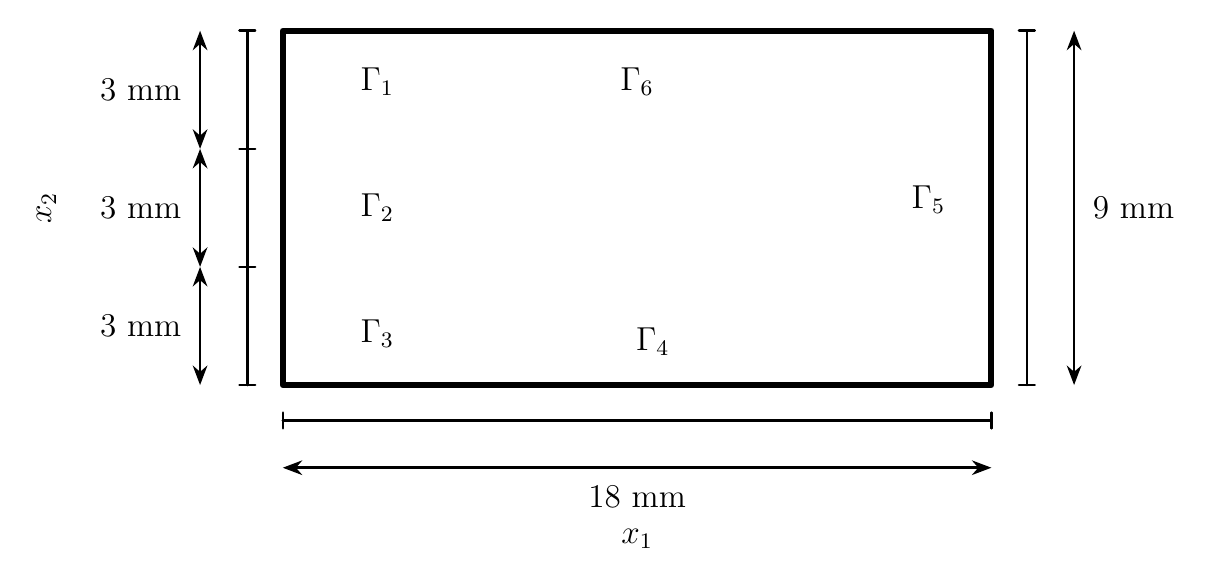
\begin{tikzpicture}[font=\large, line cap=round, line join=round]

% --- geometry (use arbitrary drawing units; labels carry "mm") ---
\def\W{9}   % width  (represents 18 mm)
\def\H{4.5} % height (represents 9  mm)

% rectangle (thick border)
\draw[line width=2.2pt] (0,0) rectangle (\W,\H);

% boundary labels
\node at (1.2,3.85) {$\Gamma_{1}$};
\node at (1.2,2.25) {$\Gamma_{2}$};
\node at (1.2,0.65) {$\Gamma_{3}$};
\node at (4.7,0.55) {$\Gamma_{4}$};
\node at (8.2,2.35) {$\Gamma_{5}$};
\node at (4.5,3.85) {$\Gamma_{6}$};

% --- dimensioning style ---
\tikzset{
  dim/.style={line width=0.9pt},
  dimArrow/.style={<->,>=Stealth,dim},
  dimTick/.style={dim}
}

% Left: three 3 mm segments (total 9 mm)
\draw[dim] (-0.45,0) -- (-0.45,\H);
\draw[dimTick] (-0.55,0) -- (-0.35,0);
\draw[dimTick] (-0.55,1.5) -- (-0.35,1.5);
\draw[dimTick] (-0.55,3.0) -- (-0.35,3.0);
\draw[dimTick] (-0.55,\H) -- (-0.35,\H);

\draw[dimArrow] (-1.05,3.0) -- (-1.05,\H)
  node[midway,left=3pt] {$3~\mathrm{mm}$};
\draw[dimArrow] (-1.05,1.5) -- (-1.05,3.0)
  node[midway,left=3pt] {$3~\mathrm{mm}$};
\draw[dimArrow] (-1.05,0) -- (-1.05,1.5)
  node[midway,left=3pt] {$3~\mathrm{mm}$};

% x2 label
\node[rotate=90] at (-3.0,2.25) {$x_{2}$};

% Right: total height 9 mm
\draw[dim] (\W+0.45,0) -- (\W+0.45,\H);
\draw[dimTick] (\W+0.35,0) -- (\W+0.55,0);
\draw[dimTick] (\W+0.35,\H) -- (\W+0.55,\H);
\draw[dimArrow] (\W+1.05,0) -- (\W+1.05,\H)
  node[midway,right=3pt] {$9~\mathrm{mm}$};

% Bottom: width 18 mm
\draw[dim] (0,-0.45) -- (\W,-0.45);
\draw[dimTick] (0,-0.35) -- (0,-0.55);
\draw[dimTick] (\W,-0.35) -- (\W,-0.55);
\draw[dimArrow] (0,-1.05) -- (\W,-1.05)
  node[midway,below=3pt] {$18~\mathrm{mm}$};

% x1 label
\node at (\W/2,-1.95) {$x_{1}$};

\end{tikzpicture}
\caption{Premixed $\HTwo$ air-flame example. Schematic of geometry and boundary conditions.}
\label{fig:air_flame_schematic}
\end{figure}


As in Ref.~\cite{GaWaZh20}, we consider two parameters: the activation energy $\mu_1 = \mathrm{E}$ and the pre-exponential factor $\mu_2=  A$. The parameter space is $\paramDomain = \left[ 2.3375 \times 10^{12} ,6.2 \times 10^{12} \right] \times \left[ 5625.5, 9000 \right].$ Note that the governing equations are nonlinear in the state and non-affine in the parameters, due to the presence of $\exp(E/R\Theta)$ in the equation for $\boldsymbol R_i$. 
The FOM is discretized with a second-order finite difference method on a $50 \times 25$ grid. We employ central differencing for diffusion and second-order upwind differencing for advection. Time integration uses second-order Crank--Nicolson with time step $1 \times 10^{-4}$, yielding $600$ snapshots per FOM sample. Figure~\ref{fig:air_flame_foms} presents FOM temperature snapshots at a randomly selected testing parameter instance. We examine the same NN-OpInf-PSD-f ROM as considered in Eq.~\eqref{eq:nnopinf_pd_f}, with the exception that the nonlinear forcing term is taken to be a fully connected feed forward neural network whose inputs are the parameters. We additionally examine P-OpInf-cA, P-OpInf-cAH, and NN-OpInf-NN models for comparison. 

We use a training/testing protocol similar to Ref.~\cite{GaWaZh20}. The training set $\paramDomainTrain$ is a uniform $4 \times 4$ grid in $\paramDomain$, while the testing set is $\paramDomainTest = \left\{ 2.98125 \times 10^{12}, 4.26875\times 10^{12},5.55625\times 10^{12} \right\} \times \left\{ 6.187917\times 10^{3},7.31275\times 10^{3},8.437583\times 10^{3} \right\}$. The only difference from Ref.~\cite{GaWaZh20} is that our testing set excludes the training samples; Ref.~\cite{GaWaZh20} used a $7 \times 7$ grid with $\paramDomainTrain \subset \paramDomainTest$.


 
\begin{figure}
\begin{center}
\begin{subfigure}[t]{0.32\textwidth}
\includegraphics[trim={0cm 0cm 0cm 0cm},clip,width=1.0\linewidth]{figs/zhar_2d_cdr/testing_solution_fom_t0.02.pdf}
\caption{$t=0.02$}
\end{subfigure}
\begin{subfigure}[t]{0.32\textwidth}
\includegraphics[trim={0cm 0cm 0cm 0cm},clip,width=1.0\linewidth]{figs/zhar_2d_cdr/testing_solution_fom_t0.04.pdf}
\caption{$t=0.04$}
\end{subfigure}
\begin{subfigure}[t]{0.32\textwidth}
\includegraphics[trim={0cm 0cm 0cm 0cm},clip,width=1.0\linewidth]{figs/zhar_2d_cdr/testing_solution_fom_t0.06.pdf}
\caption{$t=0.06$}
\end{subfigure}
\caption{Premixed $\HTwo$ air-flame example. FOM solutions for temperature at $t=0.02$ (left), $t=0.04$ (center), and $t=0.06$ (right) for $(\mu_1,\mu_2) = (5.55625 \times 10^{12},8.437583 \times 10^3)$.}
\label{fig:air_flame_foms}
\end{center}
\end{figure}

 


Figure~\ref{fig:air_flame_error} reports errors for the training set (left) and testing set (right) on the premixed $H_2$-air flame example. NN-OpInf-PSD-f outperforms NN-OpInf-NN by 5--10$\times$, and yields errors approximately an order of magnitude lower than those reported in Ref.~\cite{GaWaZh20}. Unlike the previous examples, the linear and quadratic P-OpInf models here are more accurate on the training set than NN-OpInf-PSD-f. While we note that a more accurate NN-OpInf-PSD-f ROM could be trained by tweaking the training settings, this result suggests that the polynomial terms dominate the dynamics and the use of an NN-OpInf model may be unnecessary. However, NN-OpInf-PSD-f yields slightly lower errors on the testing set than P-OpInf, demonstrating some benefit from the non-polynomial parameterization. At the highest basis dimension, NN-OpInf-PSD-f achieves roughly a $3\times$ lower error than the linear and quadratic P-OpInf models. We omit physical solution plots for these OpInf models as they are visually indistinguishable from the FOM.
 
\begin{figure}
\begin{center}
\begin{subfigure}[t]{0.49\textwidth}
\includegraphics[trim={0cm 0cm 0cm 0cm},clip,width=1.0\linewidth]{figs/zhar_2d_cdr/parametric-op-inf/error_convergence_romdim_training.pdf}
\caption{Training parameter set, $\paramDomainTrain$}
\label{fig:ex1_training_error_converge_a}
\end{subfigure}
\begin{subfigure}[t]{0.49\textwidth}
\includegraphics[trim={0cm 0cm 0cm 0cm},clip,width=1.0\linewidth]{figs/zhar_2d_cdr/parametric-op-inf/error_convergence_romdim_testing.pdf}
\caption{Testing parameter set, $\paramDomainTest$}
\label{fig:ex1_training_error_converge_a}
\end{subfigure}

\caption{Premixed $\HTwo$ air-flame example. Relative errors for various OpInf formulations as a function of ROM dimension.}
\label{fig:air_flame_error}
\end{center}
\end{figure}

\begin{comment}
\begin{figure}
\begin{center}
\begin{subfigure}[t]{0.49\textwidth}
\includegraphics[trim={0cm 0cm 0cm 0cm},clip,width=1.0\linewidth]{figs/Zhar_2d_cdr/parametric-op-inf/testing_solution_error_NNOPINF-NN.pdf}
\caption{NNOPINF-NN}
\end{subfigure}
\begin{subfigure}[t]{0.49\textwidth}
\includegraphics[trim={0cm 0cm 0cm 0cm},clip,width=1.0\linewidth]{figs/Zhar_2d_cdr/parametric-op-inf/testing_solution_error_NNOPINF-PD-f.pdf}
\caption{NNOPINF-PD-f}
\end{subfigure}
\begin{subfigure}[t]{0.49\textwidth}
\includegraphics[trim={0cm 0cm 0cm 0cm},clip,width=1.0\linewidth]{figs/Zhar_2d_cdr/parametric-op-inf/testing_solution_error_OpInf-cA.pdf}
\caption{Opinf-cA}
\end{subfigure}
\begin{subfigure}[t]{0.49\textwidth}
\includegraphics[trim={0cm 0cm 0cm 0cm},clip,width=1.0\linewidth]{figs/Zhar_2d_cdr/parametric-op-inf/testing_solution_error_OpInf-cAH.pdf}
\caption{OpInf-cAH}
\label{fig:ex1_training_error_converge_a}
\end{subfigure}
\caption{Premixed $\HTwo$ air-flame example. Relative errors for various OpInf formulations as a function of ROM dimension.}
\label{fig:air_flame_error}
\end{center}
\end{figure}
\end{comment}

%\input{radiation}
\subsection{3D hyper-elastic torsion problem}
The last application we consider arises in finite deformation solid mechanics, where the governing equations do not admit a polynomial structure for most material models. This example highlights the ability of NN-OpInf to infer a nonlinear OpInf model preserving the Lagrangian structure of the FOM. To this end, consider a body on the reference domain $\Omega \subset \RR{3}$ undergoing finite deformations described by $\boldsymbol x = \psi \left(\boldsymbol X \right)$, where $\psi : \Omega \rightarrow W$ is the deformation map, $\boldsymbol X \in \Omega$ are the reference coordinates, $\boldsymbol x \in W$ are the deformed coordinates, and $W$ is the deformed domain. The dynamics are described by the Euler--Lagrange equations
\begin{equation}\label{eq:sd}
\rho_0 \ddot{\psi} = \nabla \cdot P ,
\end{equation} 
subject to the initial conditions,
\begin{equation} \label{eq:dynamic_elasticity_bcs}
    \begin{array}{ll}
    \psi(t_0,x) = \psi_0 \quad \text{ in } \Omega, & \quad\dot{\psi}(t_0,x) = v_0 \quad \text{ in } \Omega. \\
%      \psi(t, x) = \chi \quad \text{ on } I \times \partial_{\psi}\Omega, &\quad P n = T  \quad\text{ on } I \times \partial_{T} \Omega, 
      \end{array}
\end{equation}
In the above, $\rho_0$ is the mass density and $P$ is the first Piola-Kirchhoff stress. We consider free boundary conditions in the example that follows. A Galerkin finite element discretization of Eq.~\eqref{eq:sd} yields the corresponding discrete system
$$
\mass \ddot\state   = \boldsymbol f(\state),
$$
where $\mass$ is the mass matrix and $\boldsymbol f$ are the internal forces. 
We consider a Neohookean material model with elastic modulus $1 \times 10^9$ Pa, Poisson's ratio $0.25$, and density $\rho = 1000$ kg/m$^3$. We emphasize that this material model gives rise to dynamics that are highly nonlinear, with nonlinearities that are far more complex than polynomial nonlinearities; see Appendix A.3 of \cite{TePaGr26} for details.  Moreover, the simulated dynamics are fundamentally nonlinear. 
% As a problem setup, we consider 
The problem setup models the distortion of a free beam subject to an initial velocity, which results in a high-degree of torsion; a similar example was considered in Ref.~\cite{Mota:2022, TePaGr26}. The beam is of size $0.05 \times 1.0 \times 0.05$ subject to an initial velocity profile $v_x = \alpha y z$, $v_y = \beta x z$, where $\alpha$ and $\beta$ control its magnitude. The system is discretized using (first-order) piecewise-linear polynomial elements of size $\Delta x = \Delta y = \Delta z = 0.01$ m, while time integration uses the (second-order) Newmark-$\beta$ scheme with $\Delta t = 1 \times 10^{-5}$ s, $\beta = 0.25$, and $\gamma=0.5$. 

The discretized governing equations extremize the mechanical Lagrangian,
$$\mathcal{L} ( \state,\stateDot ) = T(\stateDot) - V(\state) \coloneqq \frac{1}{2}\stateDot^T \mass \stateDot - V(\state),$$
where $T(\stateDot) = \frac{1}{2} \stateDot^T \mass \stateDot$ is the kinetic energy and $V(\state)$ is the potential energy satisfying $V'(\state) = \boldsymbol f(\state)$.  To construct an NN-OpInf ROM that maintains the Lagrangian structure of the FOM, we parameterize the right hand side with the SPSD potential operator,
\begin{equation}\label{eq:nnopinf_lagrangian}
\reducedVelocity(\reducedState,\params) =   \frac{\partial}{\partial \reducedState} \left[ \reducedState^\intercal\reducedSpdMatrixLowerNN(\reducedState,\params;\weights) \reducedSpdMatrixLowerNN^\intercal(\reducedState,\params;\weights)\reducedState \right]. 
\end{equation}
We refer to this formulation as the NN-OpInf-SPSD-Potential ROM, and note that the resulting ROM satisfies the Euler-Lagrange equations
% $$ \frac{d^2 \hat{\state}}{d t^2}  - \frac{\partial \hat{V}}{\partial \hat{\state}} = 0,$$
$$ \ddot{\reducedState}  - \hat{V}'(\reducedState) = \mathbf{0},$$
associated with the reduced Lagrangian
$$\hat{\mathcal{L}} ( \reducedState,\reducedStateDot ) = \dot\reducedState^\intercal\dot\reducedState - \hat{V}(\reducedState) \coloneqq \dot\reducedState^\intercal\dot\reducedState - \reducedState^\intercal\reducedSpdMatrixLowerNN(\reducedState,\params;\weights) \reducedSpdMatrixLowerNN^\intercal(\reducedState,\params;\weights)\reducedState.$$
This model is compared to the P-OpInf-A, P-OpInf-AH, and NN-OpInf-NN ROMs. Note that the mass matrix $\mass$ is readily available in this example, so we construct an $\mass$-orthonormal ROM basis as is standard practice. Due to the strong non-linearities in this problem, in the NN-OpInf ROMs we set the number of neurons per layer to be twice the size of the ROM dimension, $n_{\mathrm{n}} = 2K$.

Two configurations are considered:
\begin{enumerate}
\item Reproductive ROM: We set $\alpha = \beta = 7500$, collecting snapshots and making predictions over $t \in [0,2.5 \times 10^{-3}]$. Snapshots are collected at every FOM time step for a total of $250$ snapshots.
\item Future-state prediction: Using the same configuration as above, we predict over the longer interval $t \in [0,5 \times 10^{-3}]$. 
\end{enumerate}


Figure~\ref{fig:torsion_error_convergence} shows results for relative error vs basis dimension for the reproductive configuration (left) and future-state configuration (right). We observe that the NN-OpInf-SPSD-Potential model, which preserves the Lagrangian structure of the FOM, is approximately an order of magnitude more accurate that standard P-OpInf models. The vanilla NN-OpInf-NN model is unstable. Figure~\ref{fig:torsion_paraview_t0025} shows the physical space solutions for displacement for the reproductive configuration, while Figure~\ref{fig:torsion_paraview_t0050} shows results for the future-state prediction configuration. We observe that the NN-OpInf-SPSD-Potential operator faithfully approximates the FOM trajectory for the reproductive configuration and, while it differs slightly in phase as compared to the FOM in the future-state configuration, still provides a reasonable solution. While the OpInf-AH model provides a reasonable solution at the end of the reproductive regime $t=2.5 \times 10^{-3}$, it still associates with a high error and yields unphysical predictions in the future-state configuration. The linear P-OpInf-A model performs poorly for all configurations.  However, note that there exist in the literature Lagrangian and Hamiltonian structure-preserving P-OpInf formulations which may perform better than these baselines, e.g., Refs. \cite{ShKa24,ViMcGr25,GrTe23, GrTe25}. 
%While the gap between the intrusive Galerkin ROM (which we emphasize does not include hyper-reduction and does not results in a reduciton in cost) and NNOpInf-PSD-Lagrangian is  

\begin{figure}
\begin{center}
\begin{subfigure}[t]{0.49\textwidth}
\includegraphics[trim={0cm 0cm 0cm 0cm},clip,width=1.0\linewidth]{figs/torsion/convergence.pdf}
\caption{Reproductive configuration.}
\end{subfigure}
\begin{subfigure}[t]{0.49\textwidth}
\includegraphics[trim={0cm 0cm 0cm 0cm},clip,width=1.0\linewidth]{figs/torsion/convergence-future-state.pdf}
\caption{Future-state prediction.}
\end{subfigure}
\caption{Torsion problem. Relative error versus basis dimension.}
\label{fig:torsion_error_convergence}
\end{center}
\end{figure}


\begin{figure}
\begin{center}
\begin{subfigure}[t]{0.19\textwidth}
\includegraphics[trim={25cm 0cm 25cm 0cm},clip,width=1.0\linewidth]{figs/torsion/fom-t0.0025.png}
\caption{FOM}
\end{subfigure}
\begin{subfigure}[t]{0.19\textwidth}
\includegraphics[trim={25cm 0cm 25cm 0cm},clip,width=1.0\linewidth]{figs/torsion/psd-lagrangian-40-t0.0025.png}
\caption{NN-OpInf-SPSD-Potential}
\end{subfigure}
\begin{subfigure}[t]{0.19\textwidth}
\includegraphics[trim={25cm 0cm 25cm 0cm},clip,width=1.0\linewidth]{figs/torsion/linear-40-t0.0025.png}
\caption{P-OpInf-A}
\end{subfigure}
\begin{subfigure}[t]{0.19\textwidth}
\includegraphics[trim={25cm 0cm 25cm 0cm},clip,width=1.0\linewidth]{figs/torsion/quadratic-40-t0.0025.png}
\caption{P-OpInf-AH}
\end{subfigure}
\begin{subfigure}[t]{0.19\textwidth}
\includegraphics[trim={25cm 0cm 25cm 0cm},clip,width=1.0\linewidth]{figs/torsion/NN-OpInf-NN-40-t0.0025.png}
\caption{NN-OpInf-NN}
\end{subfigure}
\caption{Torsion problem. Displacement solutions at $t=2.5\times 10^{-3}$ s ($K=40$). The coloring is the displacement magnitude.}
\label{fig:torsion_paraview_t0025}
\end{center}
\end{figure}

\begin{figure}
\begin{center}
\begin{subfigure}[t]{0.19\textwidth}
\includegraphics[trim={25cm 0cm 25cm 0cm},clip,width=1.0\linewidth]{figs/torsion/fom-t0.0037.png}
\caption{FOM}
\end{subfigure}
\begin{subfigure}[t]{0.19\textwidth}
\includegraphics[trim={25cm 0cm 25cm 0cm},clip,width=1.0\linewidth]{figs/torsion/NN-OpInf-SPSD-Potential-40-t0.0037.png}
\caption{NN-OpInf-SPSD-Potential}
\end{subfigure}
\begin{subfigure}[t]{0.19\textwidth}
\includegraphics[trim={25cm 0cm 25cm 0cm},clip,width=1.0\linewidth]{figs/torsion/OpInf-A-40-t0.0037.png}
\caption{P-OpInf-A}
\end{subfigure}
\begin{subfigure}[t]{0.19\textwidth}
\includegraphics[trim={25cm 0cm 25cm 0cm},clip,width=1.0\linewidth]{figs/torsion/OpInf-AH-40-t0.0037.png}
\caption{P-OpInf-AH}
\end{subfigure}
\begin{subfigure}[t]{0.19\textwidth}
\includegraphics[trim={25cm 0cm 25cm 0cm},clip,width=1.0\linewidth]{figs/torsion/NN-OpInf-NN-40-t0.0037.png}
\caption{NN-OpInf-NN}
\end{subfigure}
%\begin{subfigure}[t]{0.19\textwidth}
%\includegraphics[trim={25cm 0cm 25cm 0cm},clip,width=1.0\linewidth]{/Users/ejparis/Research/ahead/tmp/Norma.jl/examples/ahead/single/torsion_refined/dynamic-parameterized-2/ml-models-single-7500/post-process/renders/galerkin-40-t0.0037.png}
%\caption{Galerkin ROM ($K=40$)}
%\end{subfigure}
\caption{Torsion problem. Displacement solutions at $t=3.75\times 10^{-3}$ s ($K=40$). The coloring is the displacement magnitude.}
\label{fig:torsion_paraview_t0050}
\end{center}
\end{figure}

%Figure~\ref{fig:torsion_parametric_error} reports relative error versus basis dimension for the parametric-reproductive (left) and parametric-predictive (right) settings. All OpInf-AH models are unstable, so they are omitted. The parametric-reproductive case mirrors the reproductive case: OpInf-A saturates, while NNOPINF-SPD achieves $<1\%$ error for $K > 16$. NNOPINF-SPD again outperforms the Galerkin ROM at low basis dimensions, but saturates for larger $K$. In the predictive setting, NNOPINF-SPD still outperforms OpInf-A, but errors stagnate around 2--4\% for all basis dimensions. For $K=48$, NNOPINF-SPD is an order of magnitude less accurate than the Galerkin ROM. This highlights the limitations of non-intrusive ROMs for nonlinear systems in predictive settings. 
  
  
%\begin{figure}
%\begin{center}
%\begin{subfigure}[t]{0.45\textwidth}
%\includegraphics[trim={0cm 0cm 0cm 0cm},clip,width=1.0\linewidth]{figs/torsion/parametric/error_vs_romdim_training.pdf}
%\end{subfigure}
%\begin{subfigure}[t]{0.45\textwidth}
%\includegraphics[trim={0cm 0cm 0cm 0cm},clip,width=1.0\linewidth]{figs/torsion/parametric/error_vs_romdim_testing.pdf}
%\end{subfigure}
%\caption{Torsion problem. Solutions at $t=4.0 \times 10^{-3}$ (s) for FOM (top) and various ROMs.}
%\label{fig:torsion_reproductive_error}
%\end{center}
%\end{figure}




\begin{comment}
\subsection{Shallow-ice approximation}
The second exemplar we consider is the shallow-ice approximation (SIA). The governing equations for the system on $(x,y) \in \Omega$ are given by
$$\frac{\partial H}{\partial t} + \nabla \cdot \left[ - \Gamma H^{n+2} | \nabla s |^{n-1} \nabla s \right] = m,$$
where $m$ is the surface mass balance, $s = H + b$ and $b$ is the bed elevation, $\Gamma = 2 \mathcal{A}(\rho g)^n /(n+2)$, $\rho$ is the ice density, $g$ is gravity, and $n \ge$ 1 is a positive constant integer. For spatial discretization, we employ a finite difference method in where the domain is discretized into $N_x \times N_y$ uniformly spaced nodes with spacing $\Delta x = \Delta y$. Following~\ref{cite}, we employ a staggered finite difference method. 

\EP{
\begin{enumerate}
\item No parameter variability, assess convergence with ROM dimension.
\item No parameter variability, assess future state prediction.
\item Parameter variability, assess convergence with ROM dimension on i.i.d. test set.
\end{enumerate}
}

\begin{figure}
\begin{center}
\begin{subfigure}[t]{0.49\textwidth}
\includegraphics[trim={0cm 0cm 0cm 0cm},clip,width=1.0\linewidth]{../parametric_sia_2d/example1/plots/error_convergence_romdim_training.pdf}
\end{subfigure}

\begin{subfigure}[t]{0.49\textwidth}
\includegraphics[trim={0cm 0cm 0cm 0cm},clip,width=1.0\linewidth]{../parametric_sia_2d/example1/plots/training_solution_FOM.pdf}
\caption{FOM}
\end{subfigure}
\begin{subfigure}[t]{0.49\textwidth}
\includegraphics[trim={0cm 0cm 0cm 0cm},clip,width=1.0\linewidth]{../parametric_sia_2d/example1/plots/training_solution_ROM.pdf}
\caption{Intrusive Galerkin ROM}
\end{subfigure}
\begin{subfigure}[t]{0.49\textwidth}
\includegraphics[trim={0cm 0cm 0cm 0cm},clip,width=1.0\linewidth]{../parametric_sia_2d/example1/plots/training_solution_SS-SPD.pdf}
\caption{SS-SPD}
\end{subfigure}
\begin{subfigure}[t]{0.49\textwidth}
\includegraphics[trim={0cm 0cm 0cm 0cm},clip,width=1.0\linewidth]{../parametric_sia_2d/example1/plots/training_solution_OpInf-A.pdf}
\caption{OpInf-A}
\end{subfigure}
\begin{subfigure}[t]{0.49\textwidth}
\includegraphics[trim={0cm 0cm 0cm 0cm},clip,width=1.0\linewidth]{../parametric_sia_2d/example1/plots/training_solution_OpInf-AH.pdf}
\caption{OpInf-AH}
\end{subfigure}
\begin{subfigure}[t]{0.49\textwidth}
\includegraphics[trim={0cm 0cm 0cm 0cm},clip,width=1.0\linewidth]{../parametric_sia_2d/example1/plots/training_solution_Matrix.pdf}
\caption{Matrix}
\end{subfigure}


%\begin{subfigure}[t]{0.49\textwidth}
%\includegraphics[trim={0cm 0cm 0cm 0cm},clip,width=1.0\linewidth]{../parametric_advection_diffusion/example4/plots/training_solution.png}
%\end{subfigure}
%\caption{Example 1, nonlinear advection-diffusion-reaction system. Loss function evaluated on training and validation sets for various inference architectures.}
\label{fig:ex1_training_error_converge}
\end{center}
\end{figure}

\end{comment}
\section{Conclusions}\label{sec:conclusions}
We presented NN-OpInf: a neural-network-based, structure-preserving, composable OpInf framework for non-intrusive reduced-order modeling. The approach learns a latent dynamics model from snapshot data by parameterizing a reduced velocity field with a sum of neural-network-based operators, each admitting a specified algebraic structure (e.g., skew-symmetry). The approach captures complex dynamics while preserving key local structure, providing a flexible mechanism for blending heterogeneous operator blocks while maintaining interpretability and physical constraints at the component level. We outlined the mathematical formulation of the approach as well as the open-source \code{NN-OpInf} software package in which the approach is implemented. 

We analyzed computational cost and convexity properties of NN-OpInf, including explicit FLOP comparisons against linear and quadratic P-OpInf and convexity results for linear structured operators. This analysis shows that the computational cost of the forward pass of NN-OpInf models is on the same order of magnitude as that for quadratic P-OpInf models, and that the primary increase in cost from NN-OpInf occurs in the (offline) training phase.  
This is due to NN-OpInf inference problems being non-convex in general, requiring iterative batch gradient-descent optimization algorithms where many forward and adjoint passes are executed.  However, note that this relative increase in training cost over P-OpInf reduces for large basis dimensions, while the online costs remain comparable to global quadratic models of the same dimension.  Moreover, NN-OpInf ROMs are more general, as they are capable of capturing generic nonlinearities.

% The relative increase in training cost as compared to quadratic OpInf reduces for large basis dimensions, however. 

Numerical experiments across several nonlinear and parametric systems demonstrate that the structured NN-OpInf models consistently improve accuracy and robustness relative to P-OpInf and vanilla neural network baselines, particularly in predictive regimes. The results also show that enforcing structure can stabilize ROM performance and improve generalization when polynomial structure is not adequate. Future work will focus on improved optimization strategies, richer operator libraries, dynamics-constrained training, uncertainty quantification for ROM predictions, and extensions to additional multiphysics systems.

\section{Acknowledgements}
Support for this work was received through Sandia National Laboratories’ Laboratory Directed Research
and Development (LDRD) program and through the U.S. Department of Energy, Office of Science,
Office of Advanced Scientific Computing Research, Mathematical Multifaceted Integrated Capability
Centers (MMICCs) program, under Field Work Proposal 22025291 and the Multifaceted Mathematics for
Predictive Digital Twins (M2dt) project. Additionally, the writing of this manuscript was funded in part
by Irina Tezaur’s Presidential Early Career Award for Scientists and Engineers (PECASE).
Sandia National Laboratories is a multi-mission laboratory managed and
operated by National Technology \& Engineering Solutions of Sandia, LLC
(NTESS), a wholly owned subsidiary of Honeywell International Inc.,
for the U.S. Department of Energy's National Nuclear Security
Administration (DOE/NNSA) under contract DE-NA0003525. This written
work is authored by an employee of NTESS. The employee, not NTESS,
owns the right, title and interest in and to the written work and is
responsible for its contents. Any subjective views or opinions that
might be expressed in the written work do not necessarily represent
the views of the U.S. Government. The publisher acknowledges that the
U.S. Government retains a non-exclusive, paid-up, irrevocable,
world-wide license to publish or reproduce the published form of this
written work or allow others to do so, for U.S. Government
purposes. The DOE will provide public access to results of federally
sponsored research in accordance with the DOE Public Access Plan.

\section{Declaration on the Use of Generative AI}
In preparing this manuscript, the authors used generative AI for manuscript formatting, assistance with table generation, general manuscript editing and review, and code documentation.

\input{spd-opinf.bbl}

\end{document}
